\section{Pendahuluan}
\subsection{Latar Belakang}
Digital to Analog Converter (DAC) adalah perangkat yang berfungsi untuk mengubah sinyal digital menjadi sinyal analog. 
Sinyal digital yang dihasilkan oleh komputer atau mikrokontroler Arduino harus dapat diubah menjadi sinyal analog untuk dapat digunakan dalam berbagai aplikasi, seperti penggunaan dalam sistem audio, pengukuran, dan lain-lain.
\\\\
Prinsip kerja DAC melibatkan proses penggunaan resistor yang berat sebelah (binary weighted resistors) atau jaringan resistor R-2R ladder untuk menghasilkan output analog yang sesuai dengan input digital. 
Metode ini memungkinkan DAC untuk menghasilkan sinyal analog yang akurat dengan menggunakan kombinasi bit-bit digital.
\\\\
Dalam sistem monitoring, DAC digunakan untuk mengubah sinyal digital dari sensor menjadi sinyal analog yang dapat diproses oleh sistem. 
Misalnya, dalam pengukuran suhu, sensor suhu menghasilkan sinyal digital yang kemudian dikonversi menjadi sinyal analog oleh DAC sebelum diproses oleh sistem. 
Hal ini menunjukkan bahwa DAC sangat penting dalam sistem monitoring untuk mengubah sinyal digital menjadi sinyal analog yang dapat diproses oleh komputer.
\\\\

\subsection{Maksud dan Tujuan}
Mengetahui dan membandingkan hasil dari digital to analog converter pada Arduino dan Osiloskop.

\subsection{Hasil yang diharapkan}
Mendapatkan kesimpulan perbandingan hasil digital to analog converter pada Arduino dan Osiloskop.
%===========================================================%
\section{Tugas Pendahuluan}
\begin{center}
	\colorbox{cyan!30}{\parbox{0.8\linewidth}{
    \begin{enumerate}
        \item Apa yang dimaksud dengan Simple Queue?
        \item Keuntungan apa yang bisa didapat jika diterapkan ke suatu network?
    \end{enumerate}}}
\end{center}

%===========================================================%
\section{Alat dan Bahan}
\begin{itemize}[label=$\bullet$, itemsep=-1pt, leftmargin=*]
	\item 1 RouterOS mikrotik
	\item 2 Laptop
	\item Kabel LAN
	\item Software Winbox
\end{itemize}

%===========================================================%
\section{Jangka Waktu Pelaksanaan}
Pemahaman dan konfigurasi 1 jam.

%===========================================================%
\section{Penjelasan dan Tahapan Konfigurasi}

%======================PERCOBAAN 1==========================%
\subsection{Percobaan 1}
\begin{center}
    \begin{enumerate}
        \item Buka aplikasi Winbox pada PC dan lakukan hubungkan ke Router. Pastikan Login terisi “admin”, Klik Neighbors > Klik Refresh > Pilih Router yang ingin disambungkan > Klik Connect.
        \begin{figure}[H]
			\centering
			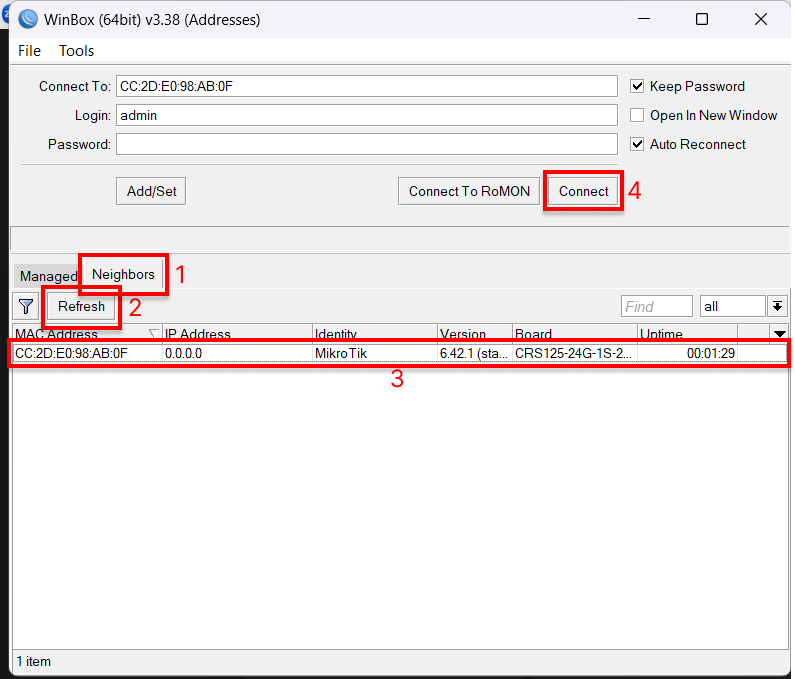
\includegraphics[width=0.5\linewidth]{P3/img/Step 1.png}
			\caption{Step 1}
			\label{fig:Step 1}
		\end{figure}
        \item Jadikan Router menjadi DHCP Client agar bisa mendapat IP address dari Internet ITS. IP > Klik DHCP Client > Tambahkan DHCP Client > Pilih interface yang terhubung dengan Internet (ether6)> Klik Apply > Klik OK.
        \begin{figure}[H]
			\centering
			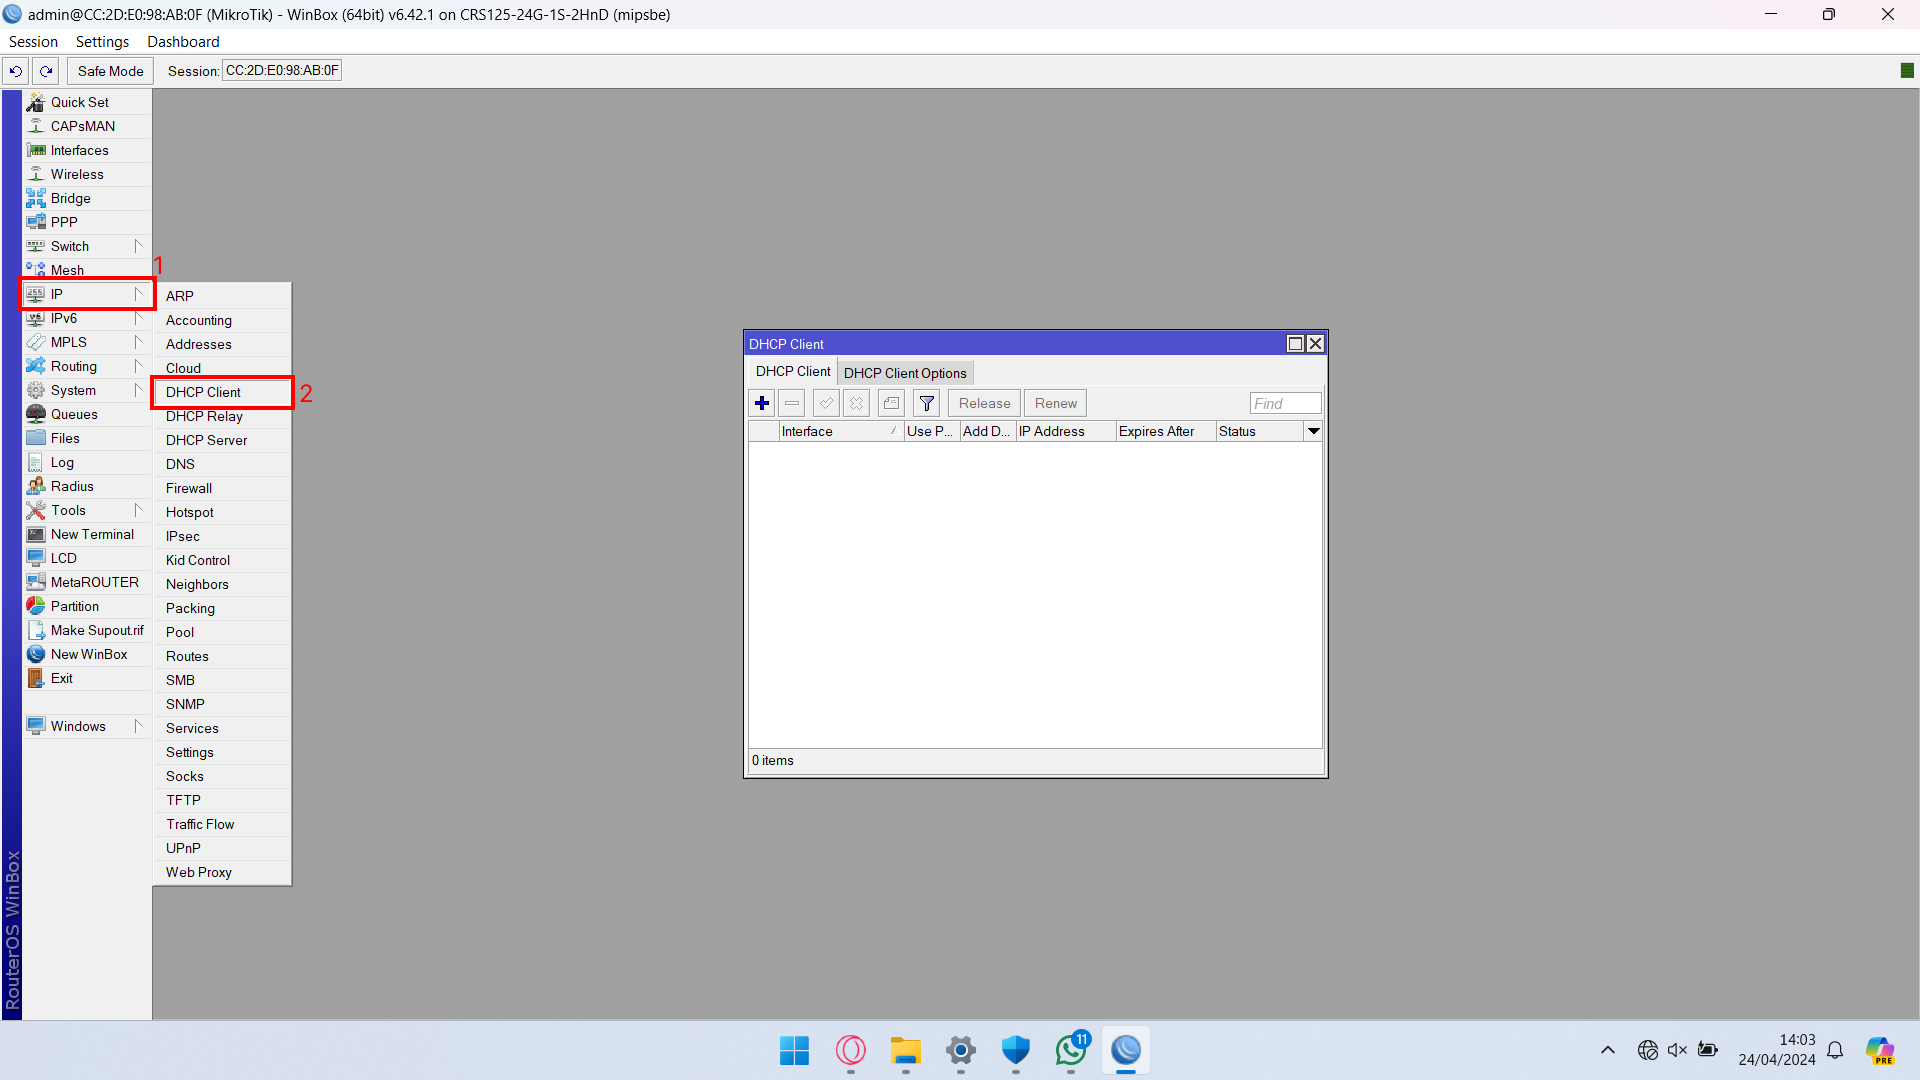
\includegraphics[width=0.8\linewidth]{P3/img/Step 2.1.png}
			\caption{Step 2.1}
			\label{fig:Step 2.1}
		\end{figure}
        \begin{figure}[H]
			\centering
			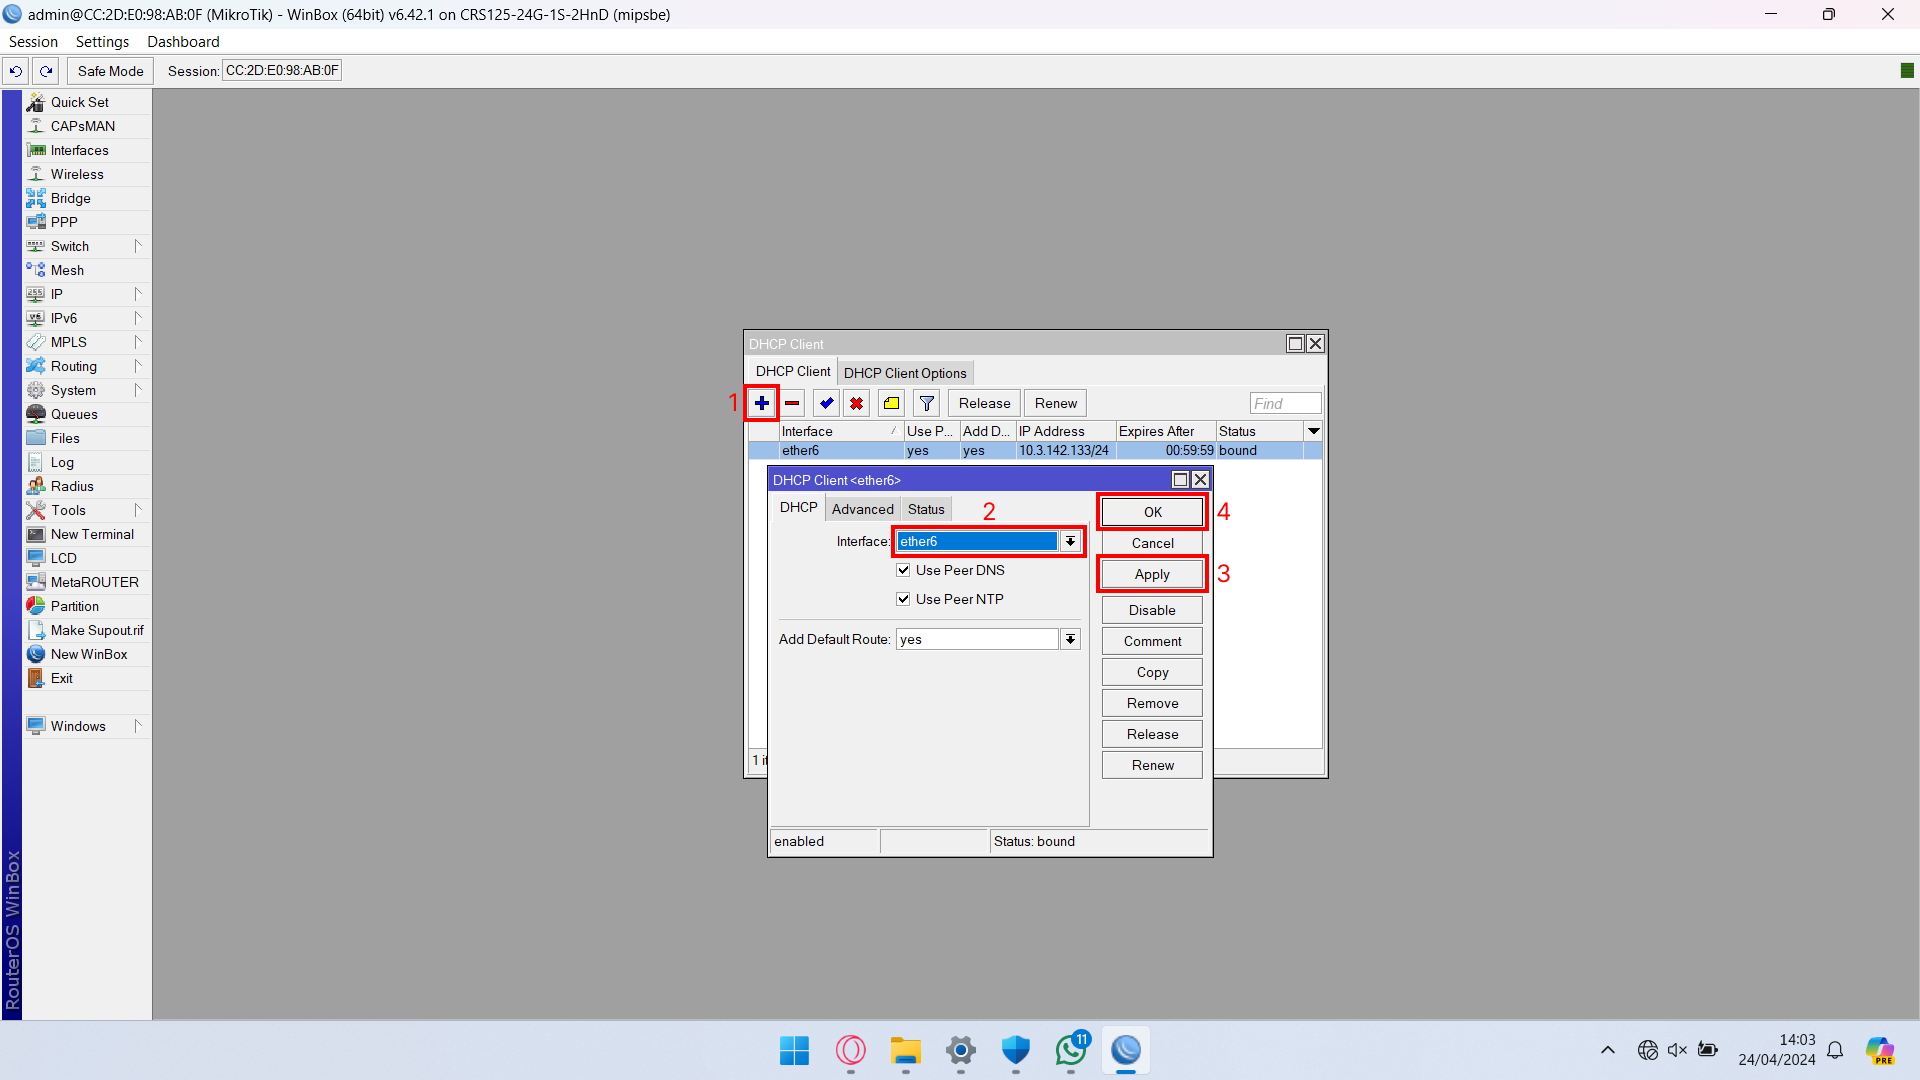
\includegraphics[width=0.8\linewidth]{P3/img/Step 2.2.png}
			\caption{Step 2.2}
			\label{fig:Step 2.2}
		\end{figure}
        \item Buat IP address pada Router yang menghubungkan PC dengan Router. Tambahkan IP address > Isi address > Pilih Interface yang terhubung ke PC (ether2) > Klik Apply > Klik OK.
        \begin{figure}[H]
			\centering
			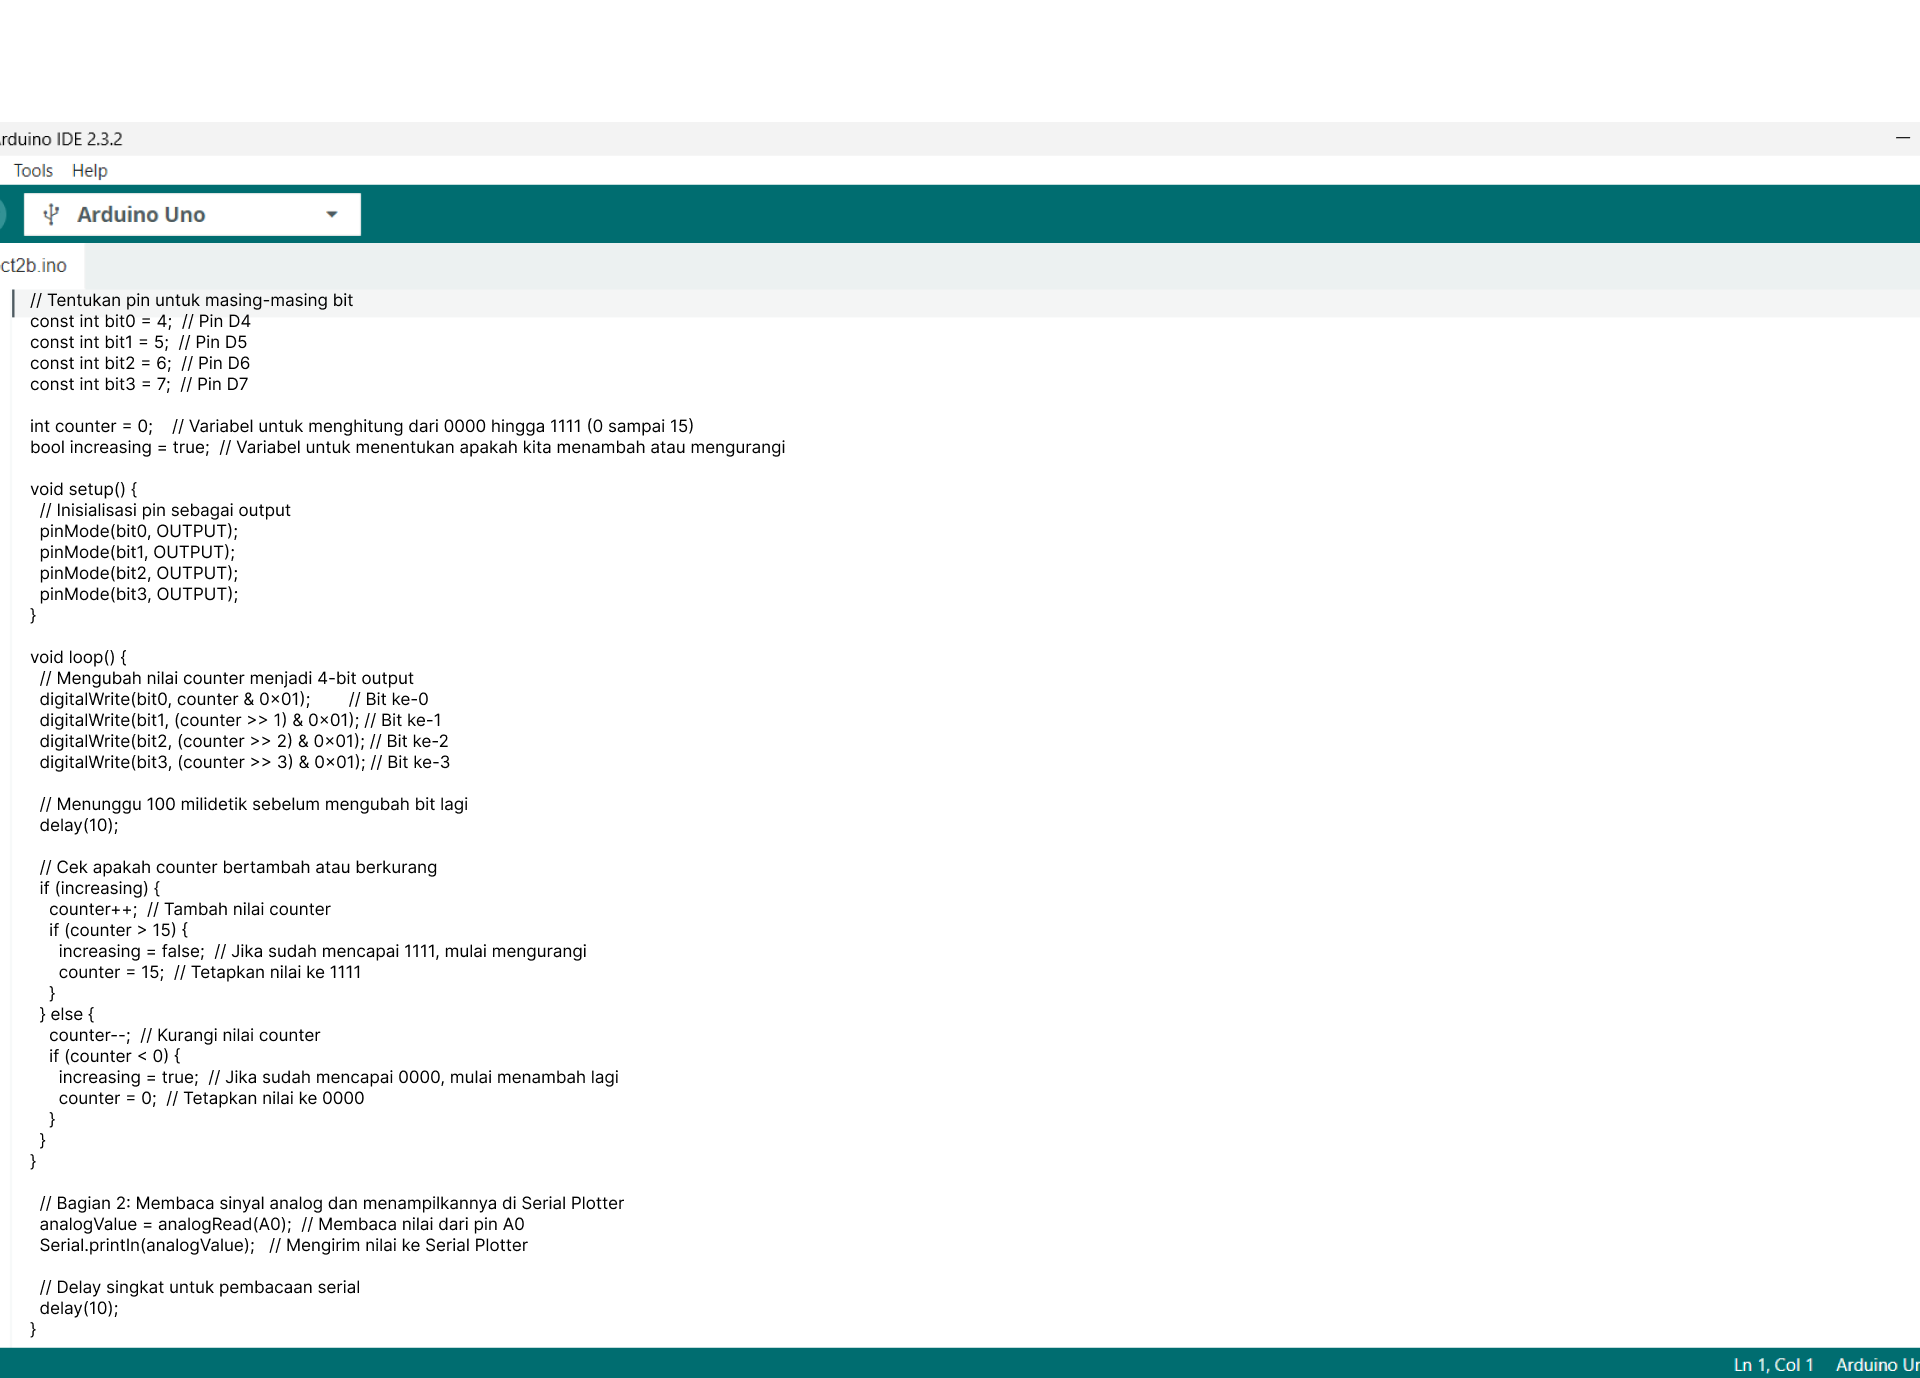
\includegraphics[width=0.8\linewidth]{P3/img/Step 3.png}
			\caption{Step 3}
			\label{fig:Step 3}
		\end{figure}
        \item Jadikan Router menjadi DHCP Server agar bisa memberikan IP address secara DInamis kepada perangkat yang akan terhubung ke Router. IP > Klik DHCP Server
        \begin{figure}[H]
			\centering
			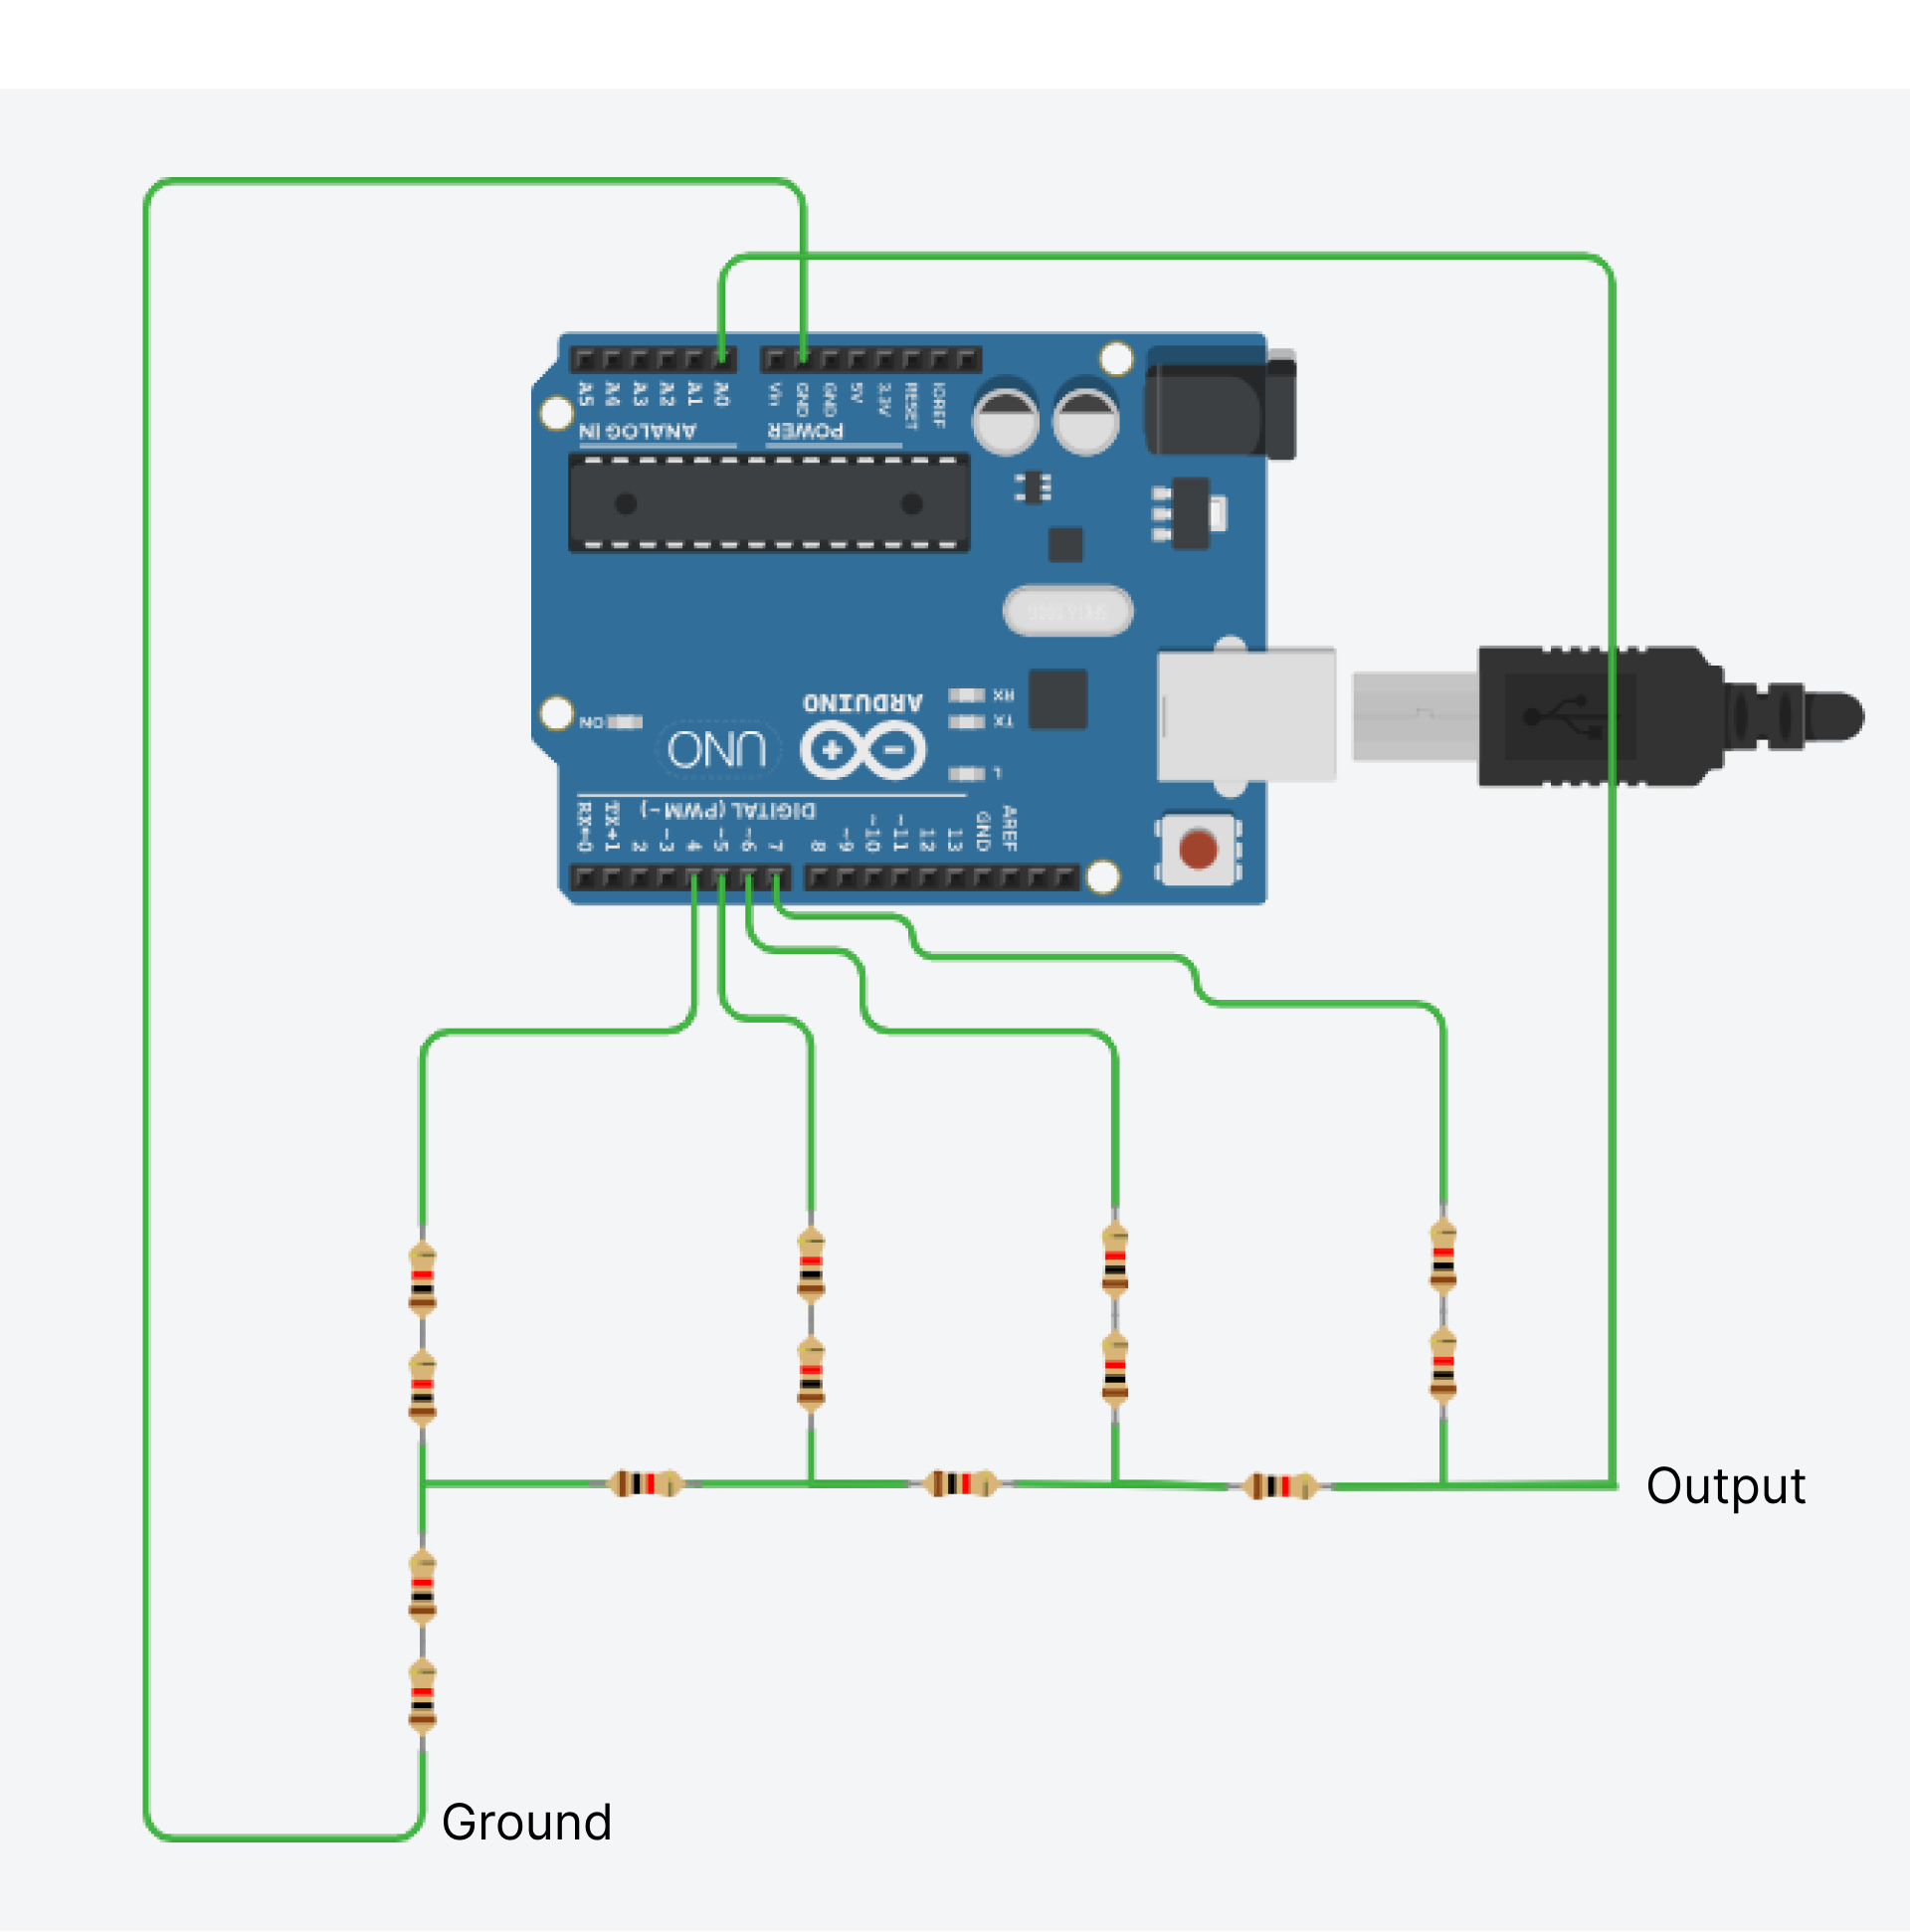
\includegraphics[width=0.8\linewidth]{P3/img/Step 4.png}
			\caption{Step 4}
			\label{fig:Step 4}
		\end{figure}
        \item Untuk menjadikan Router menjadi DHCP Server ada beberapa parameter yang harus di buat. Parameter pertama adalah DHCP Server Interface yang akan menjadi port Output DHCP Server. Klik DHCP Setup > Pilih Interface yang yang akan menjadi Server (ether2).
        \begin{figure}[H]
			\centering
			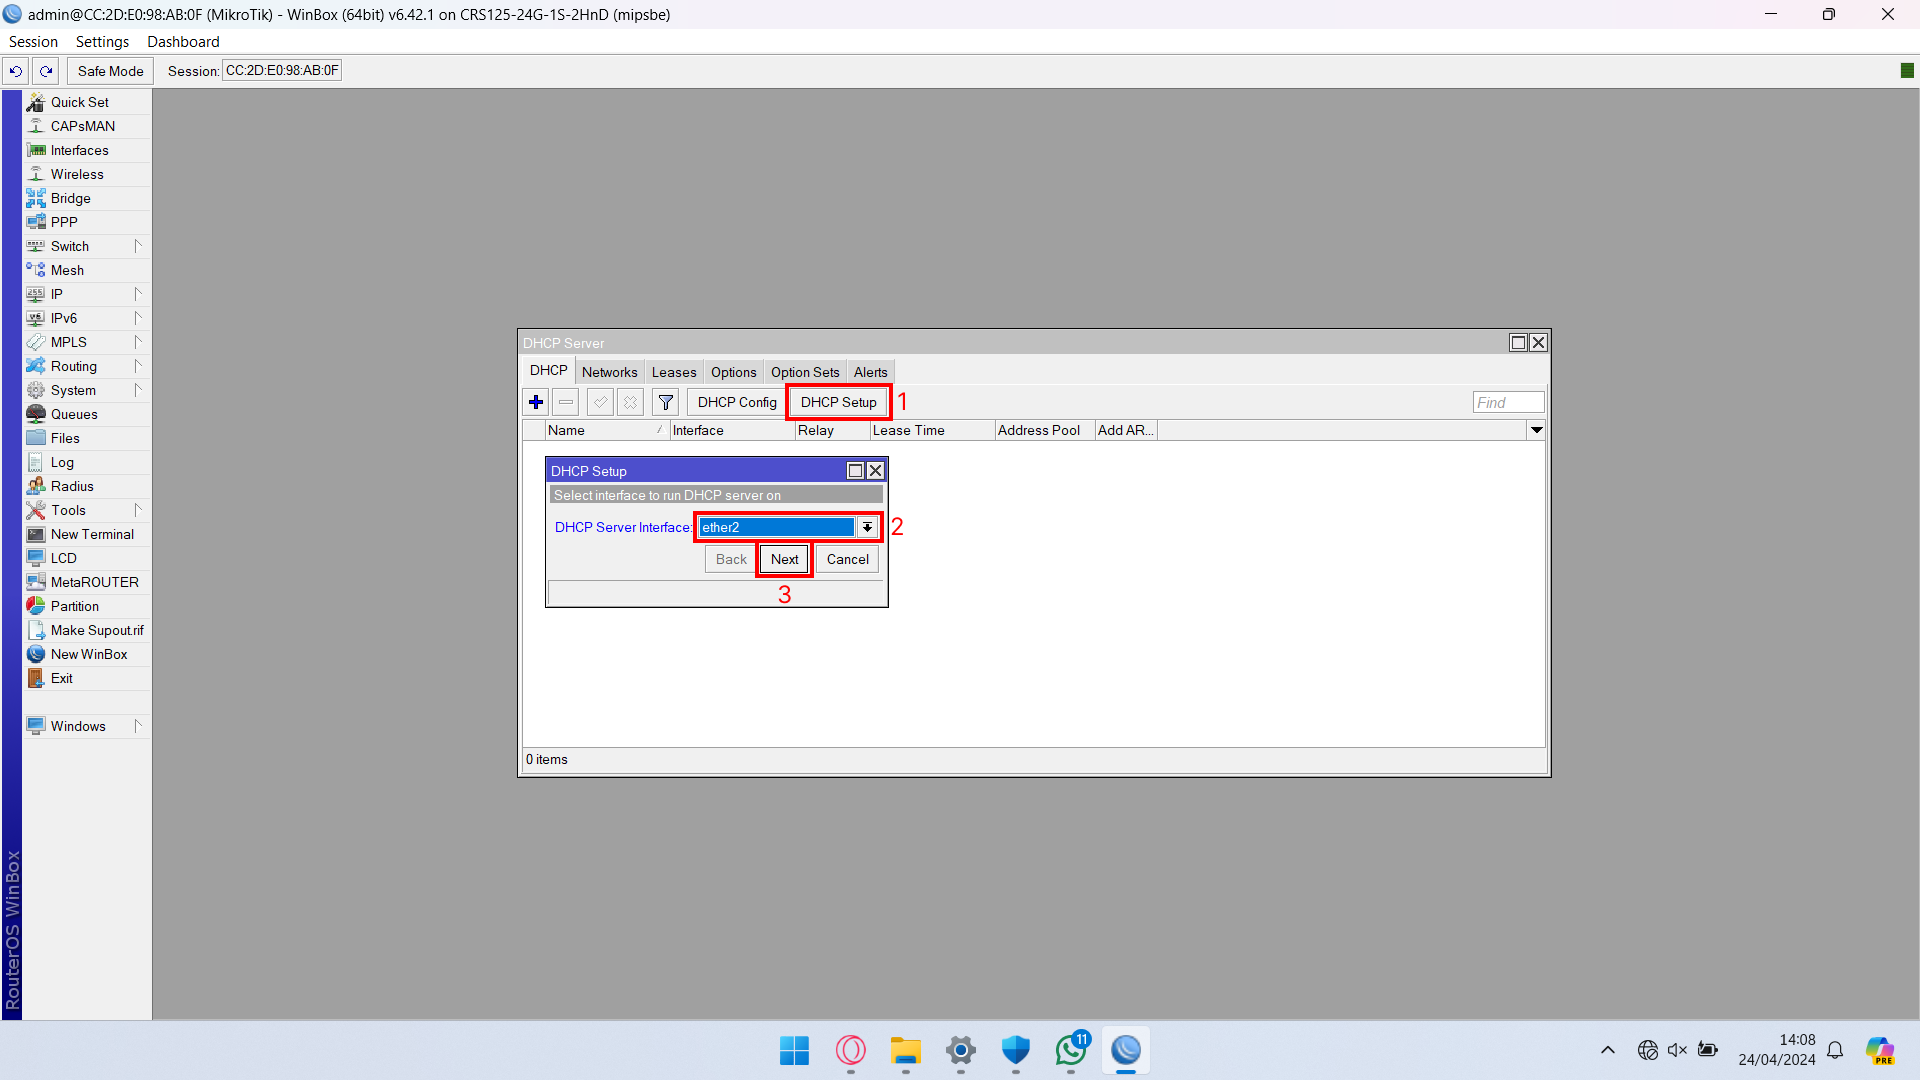
\includegraphics[width=0.8\linewidth]{P3/img/Step 5.png}
			\caption{Step 5}
			\label{fig:Step 5}
		\end{figure}
        \item Parameter kedua adalah DHCP Address Space. Isinya adalah alamat Network yang ingin dibuat. Oleh karena itu alamat IP nya diakhiri dengan angka 0.
        \begin{figure}[H]
			\centering
			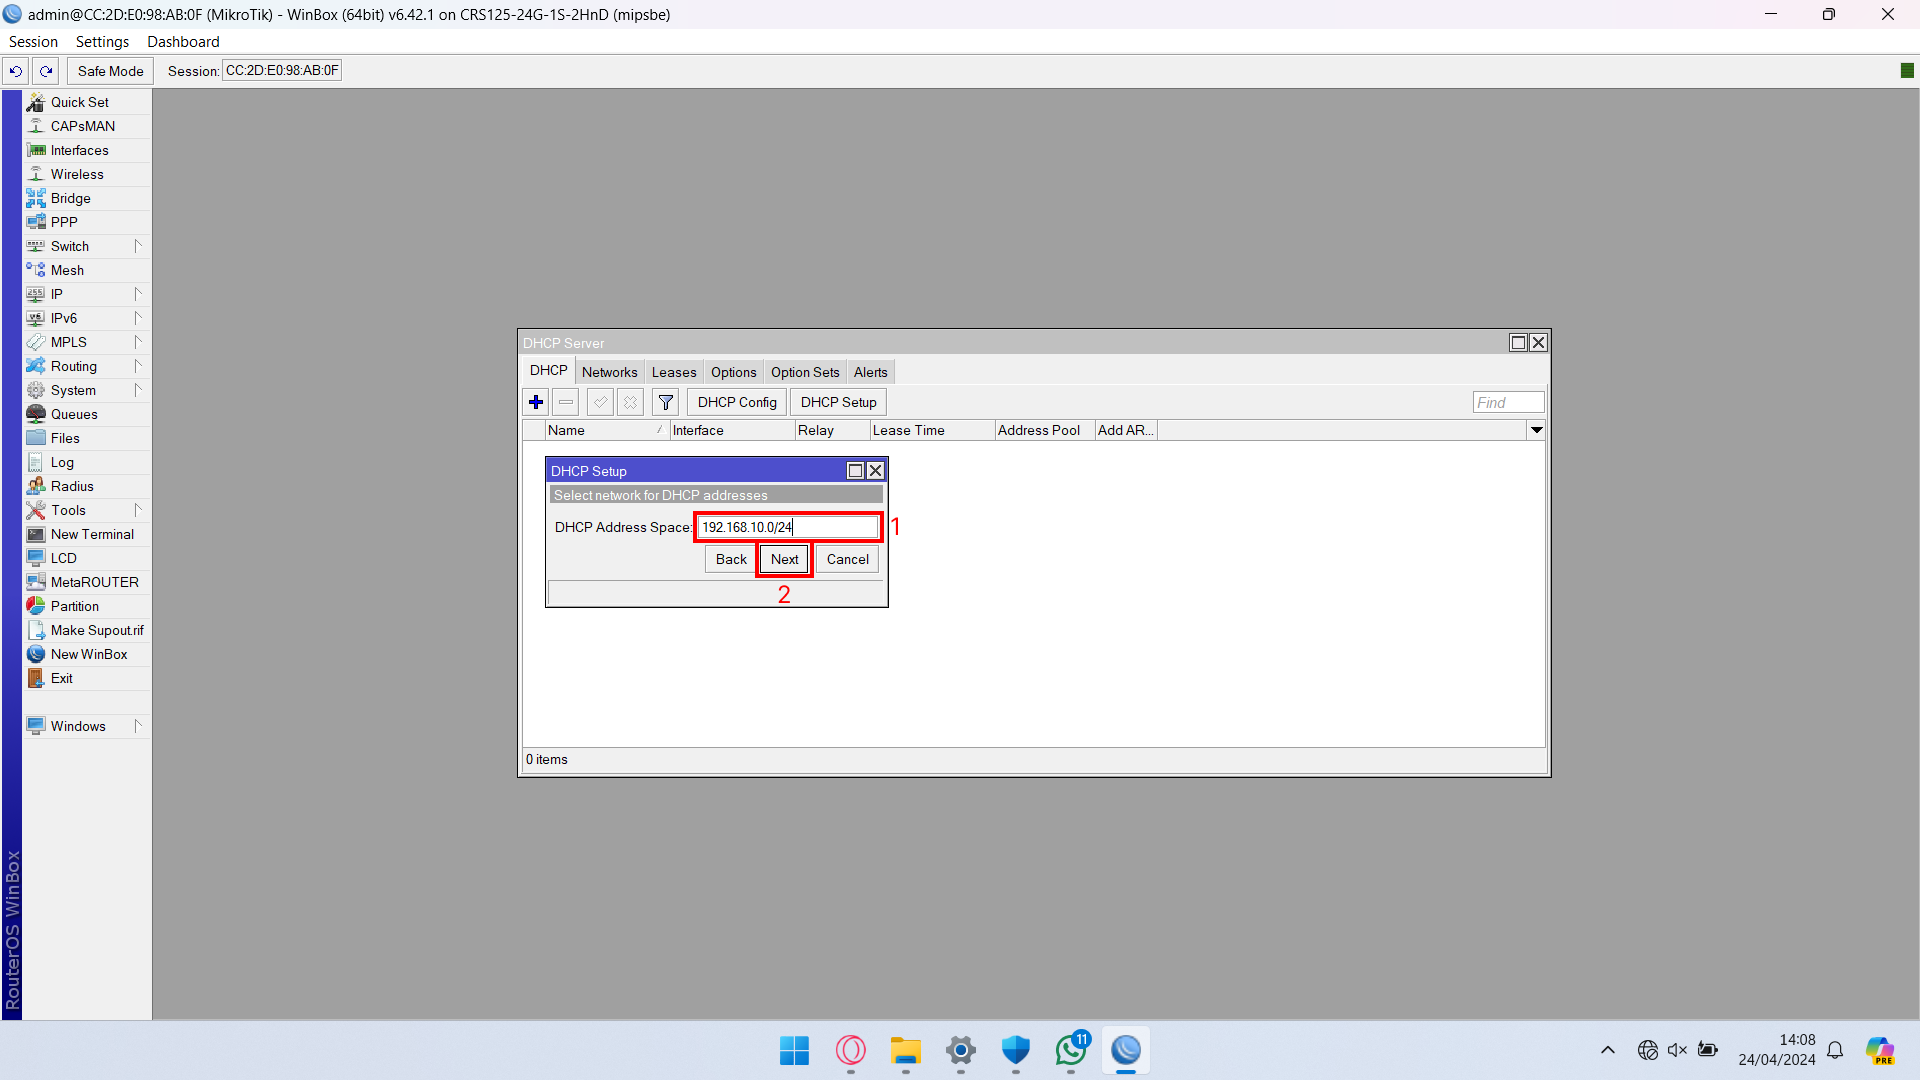
\includegraphics[width=0.8\linewidth]{P3/img/Step 6.png}
			\caption{Step 6}
			\label{fig:Step 6}
		\end{figure}
        \item Parameter ketiga adalah Gateway for DHCP Network. Isinya adalah port pada Router yang akan menghubungkan Router dengan Network address yang sudah ditentukan.
        \begin{figure}[H]
			\centering
			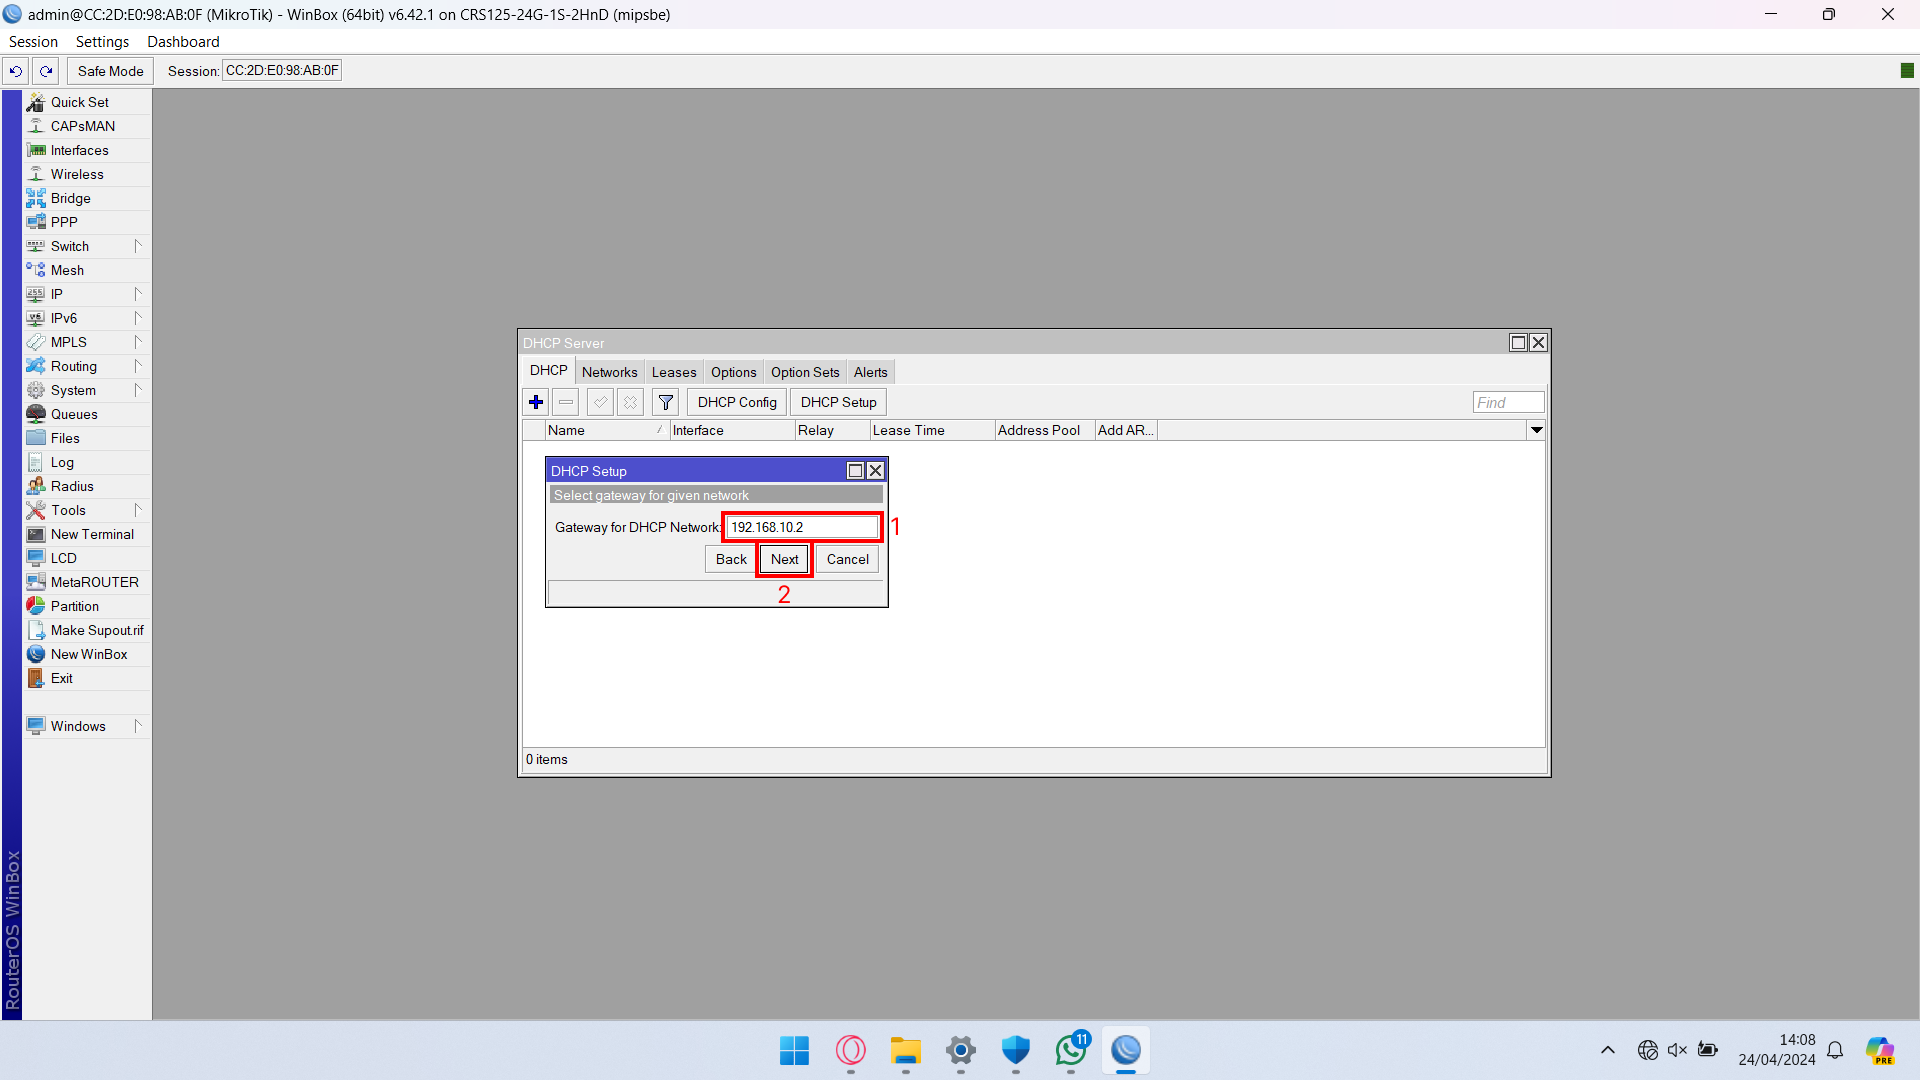
\includegraphics[width=0.8\linewidth]{P3/img/Step 7.png}
			\caption{Step 7}
			\label{fig:Step 7}
		\end{figure}
        \item Parameter keempat adalah Adresses to Give Out. Isinya adalah range IP address yang akan diberikan kepada masing-masing perangkat yang akan terhubung. Pada Modul alamat yang dapat diberikan adalah antara 192.168.10.3 sampai 192.168.10.255.
        \begin{figure}[H]
			\centering
			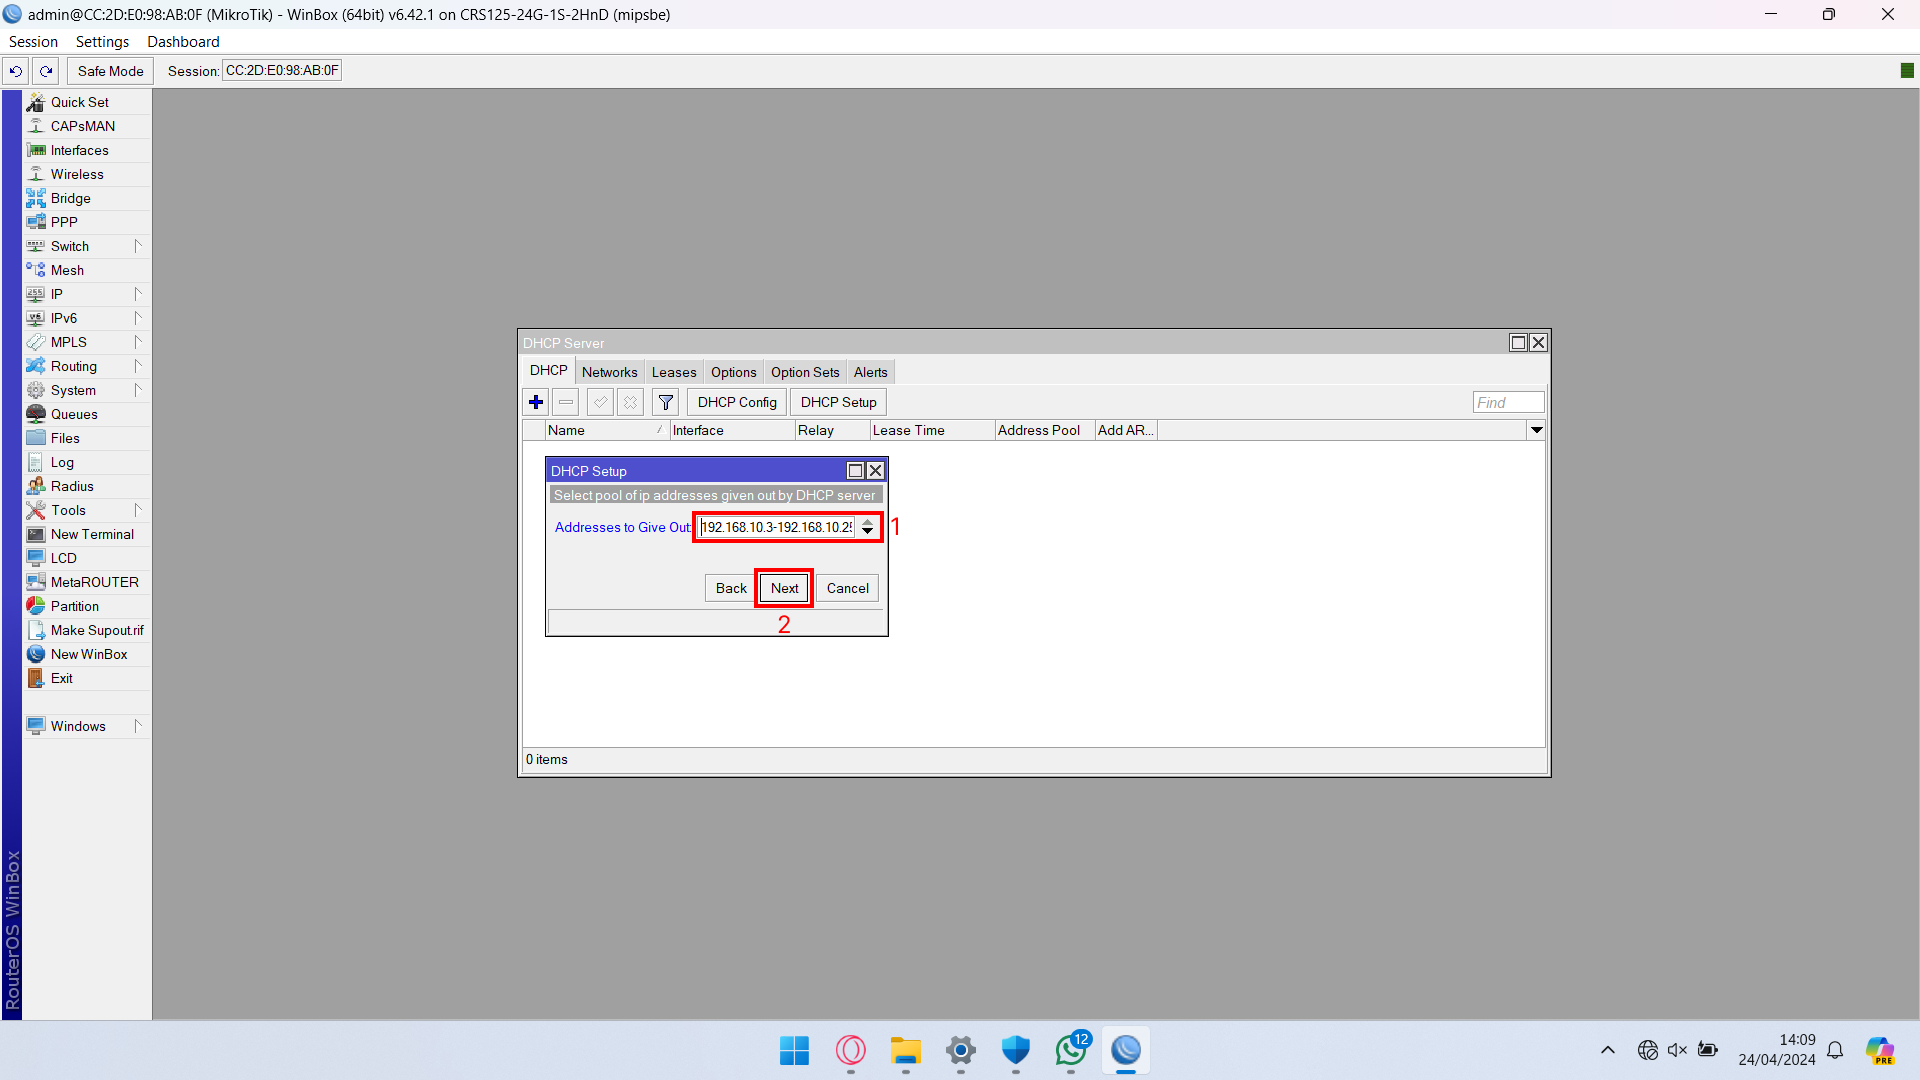
\includegraphics[width=0.8\linewidth]{P3/img/Step 8.png}
			\caption{Step 8}
			\label{fig:Step 8}
		\end{figure}
        \item Parameter kelima adalah DNS Servers. Untuk opsi langsung saja Klik Next.
        \begin{figure}[H]
			\centering
			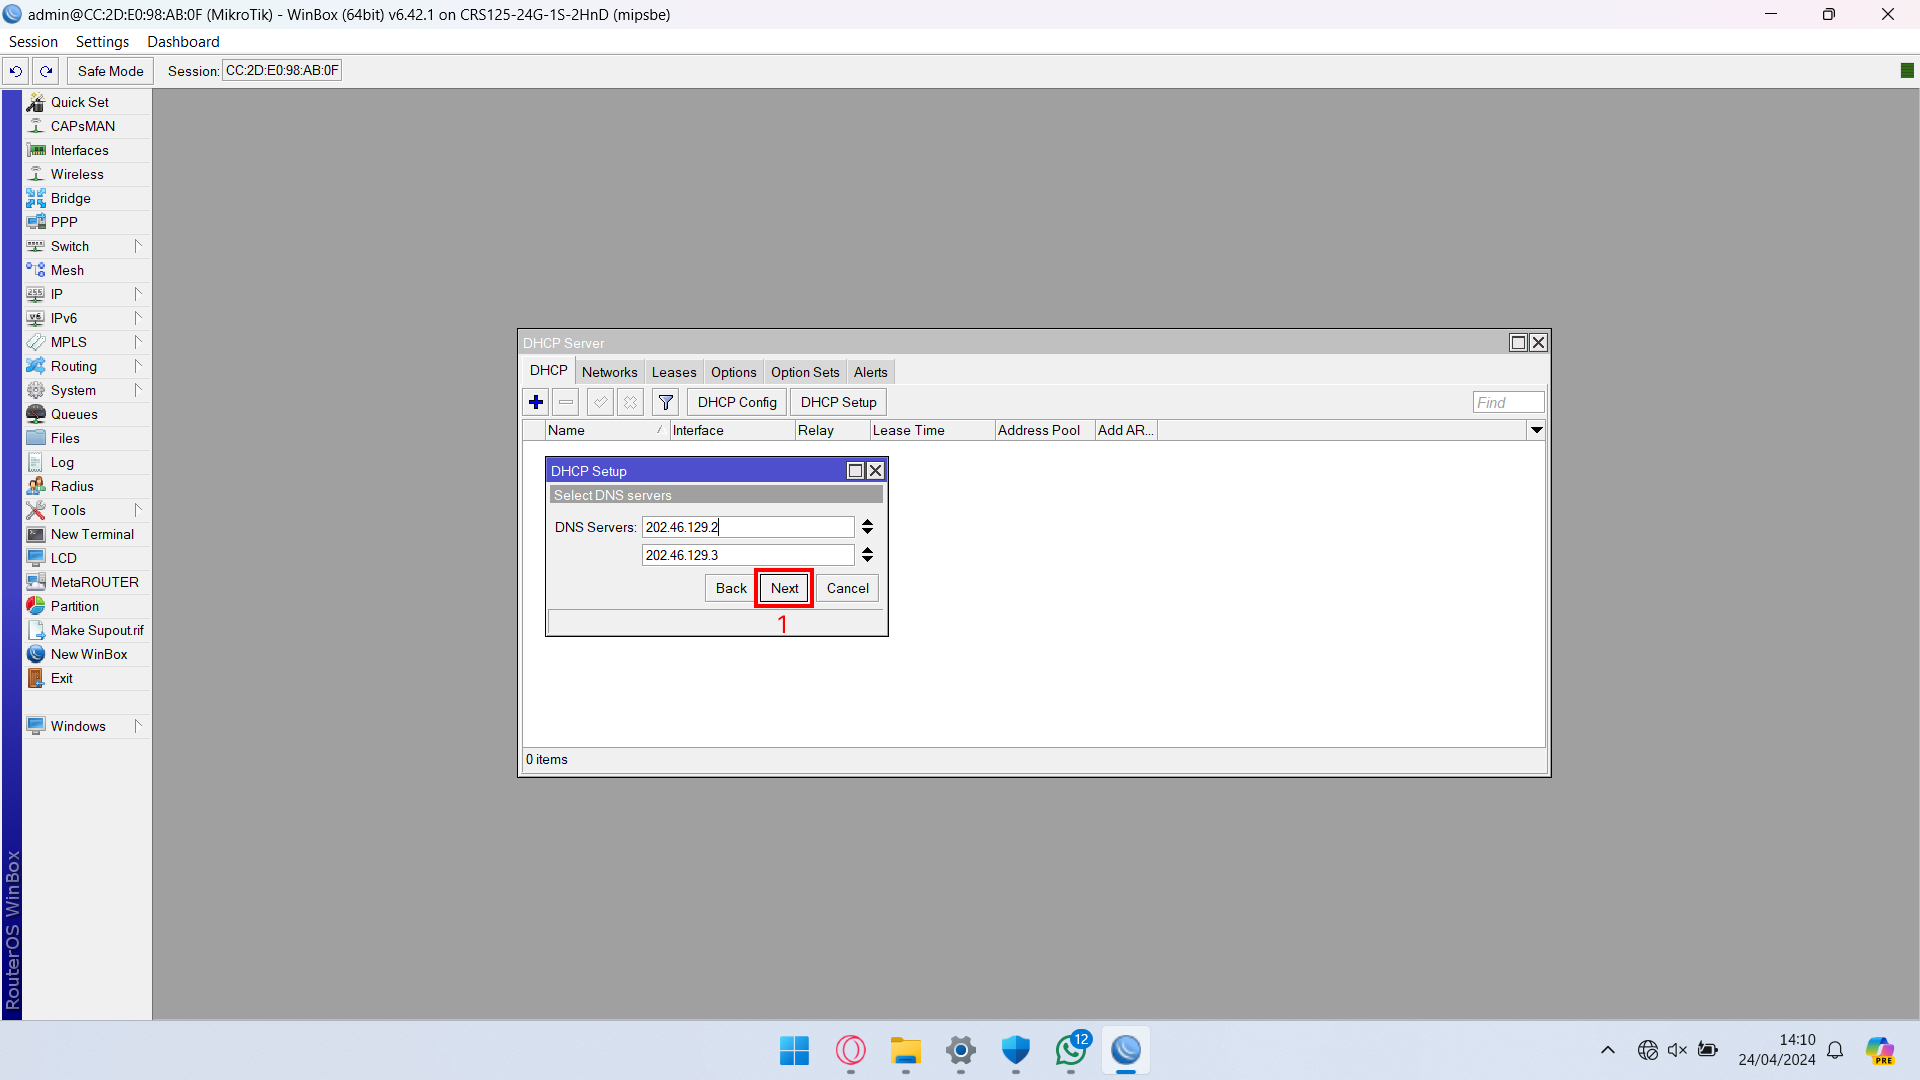
\includegraphics[width=0.8\linewidth]{P3/img/Step 9.png}
			\caption{Step 9}
			\label{fig:Step 9}
		\end{figure}
        \item Parameter keenam adalah Lease Time. Lease Time dipakai untuk membatasi waktu penggunaan IP address yang diberikan oleh Router kepada Devices. Untuk opsi langsung saja Klik Next.
        \begin{figure}[H]
			\centering
			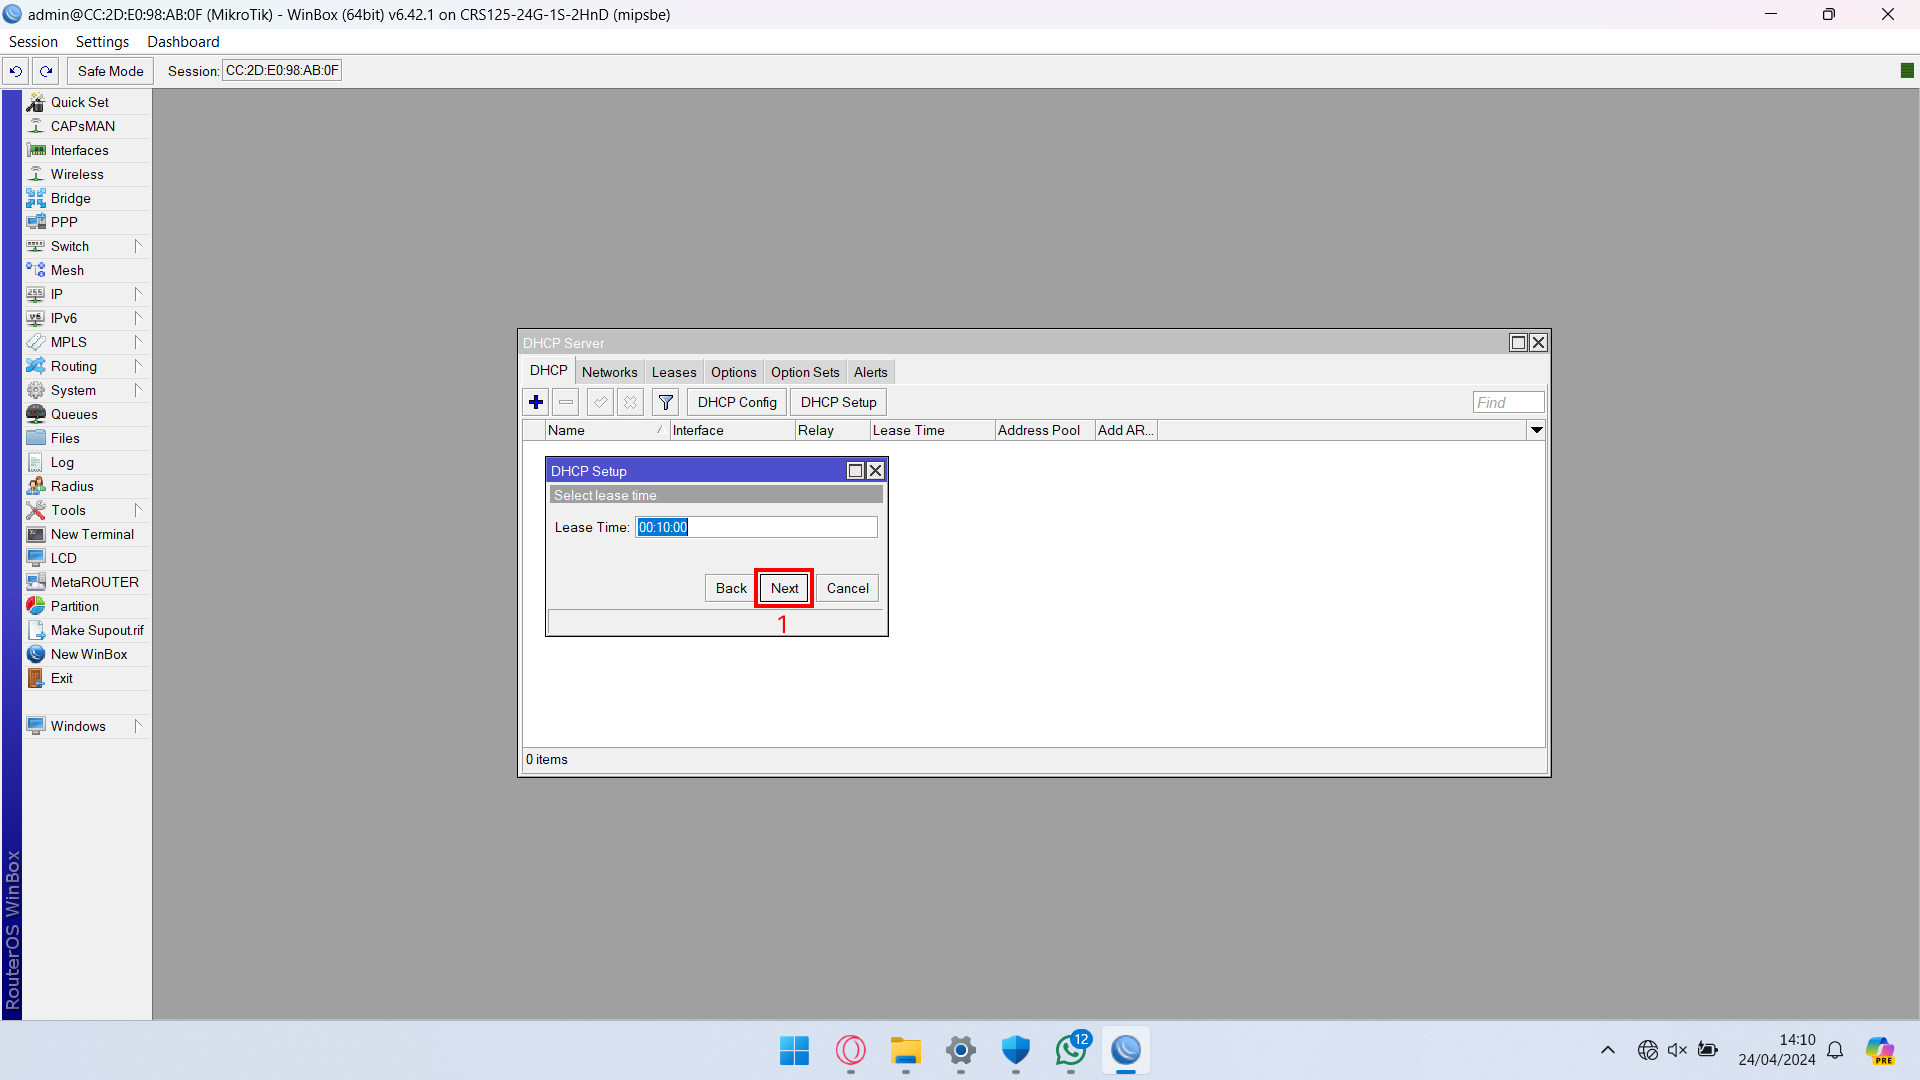
\includegraphics[width=0.8\linewidth]{P3/img/Step 10.png}
			\caption{Step 10}
			\label{fig:Step 10}
		\end{figure}
        \item Pastikan IP Settings untuk koneksi Ethernet pada PC sudah pada Mode Automatic (DHCP).
        \begin{figure}[H]
			\centering
			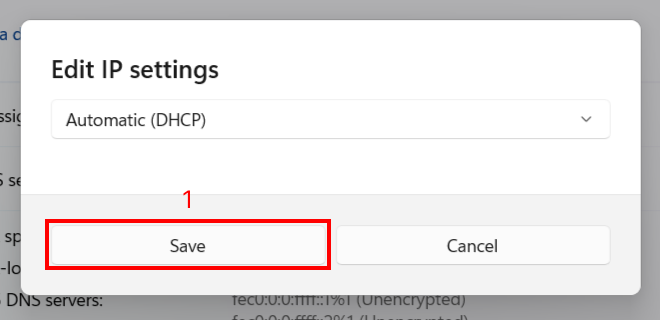
\includegraphics[width=0.8\linewidth]{P3/img/Step 11.png}
			\caption{Step 11}
			\label{fig:Step 11}
		\end{figure}
        \item Agar PC yang berada pada jaringan lokal dapat terhubung ke jaringan publik, dapat digunakan layanan NAT (Network Address Translation) yang akan menerjemahkan IP lokal beserta port perangkat agar dapat terhubung dengan jaringan publik. IP > Klik Firewall.
        \begin{figure}[H]
			\centering
			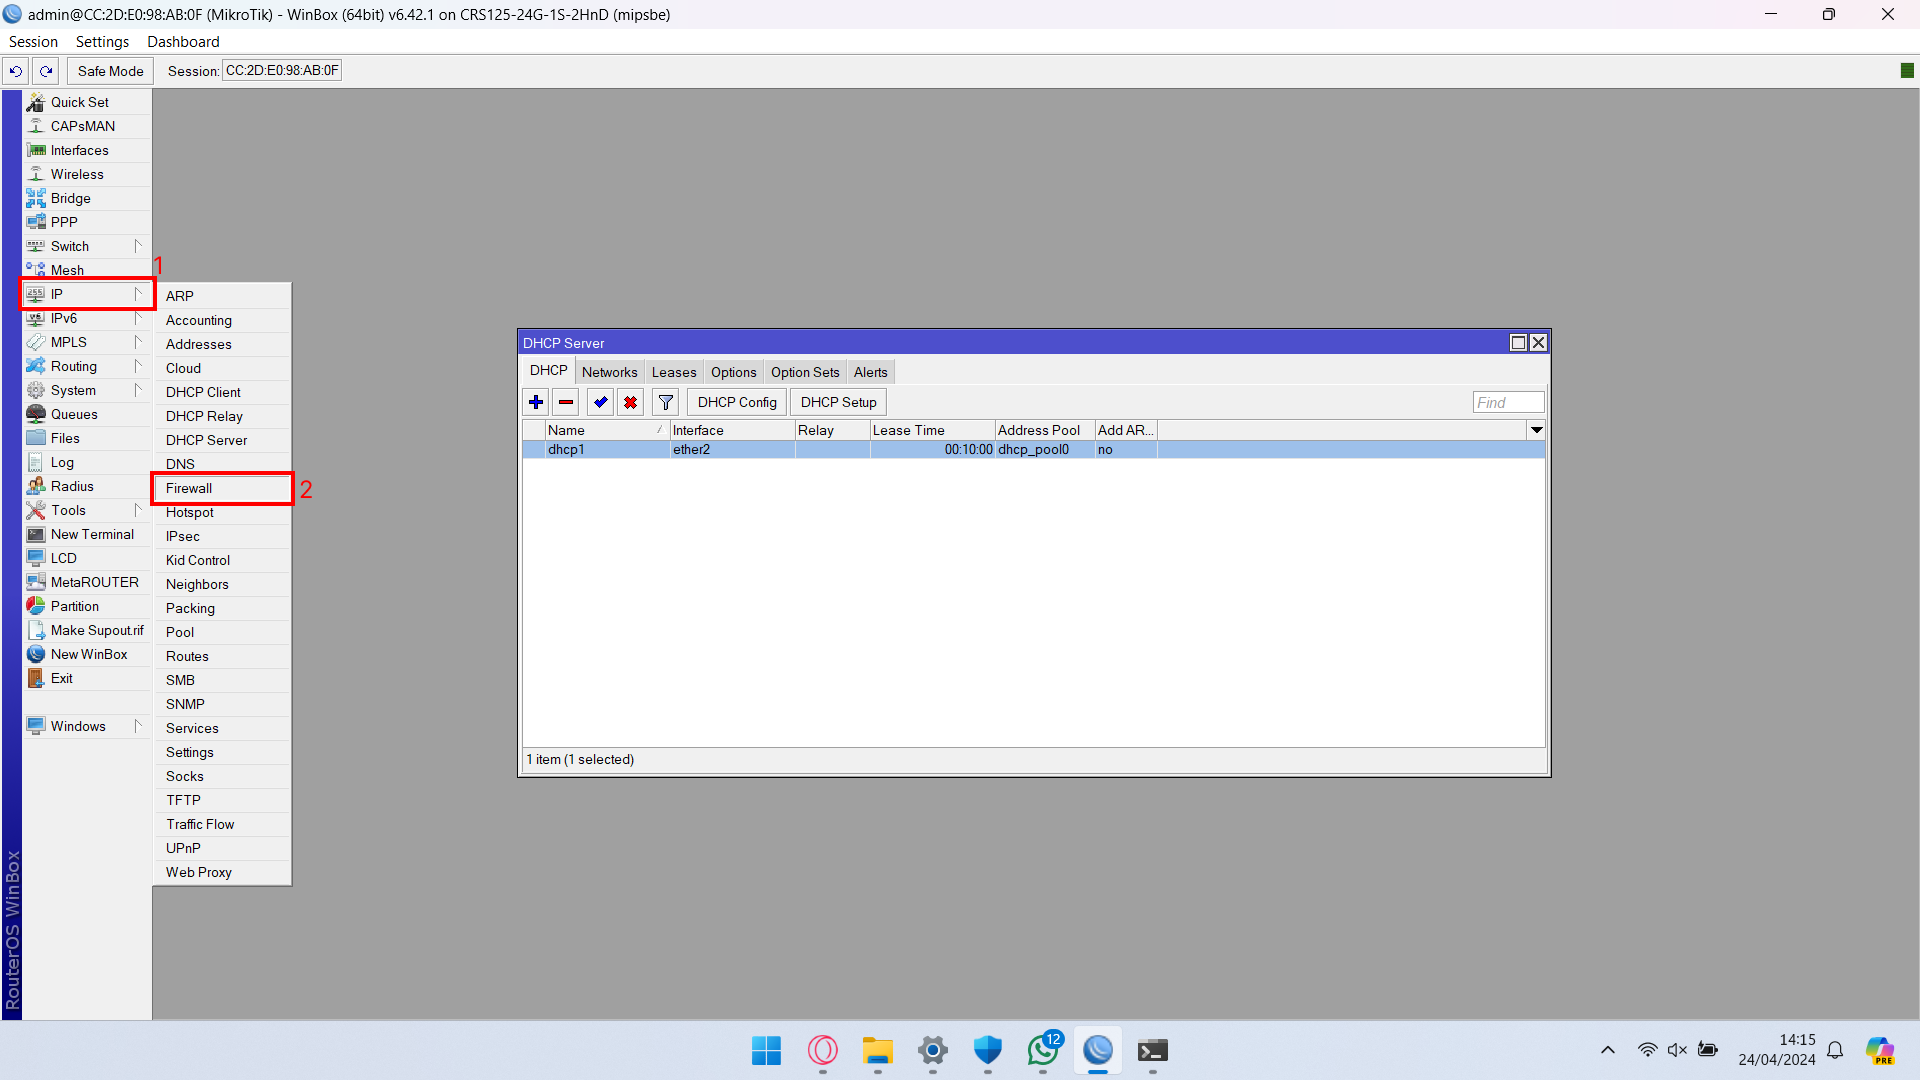
\includegraphics[width=0.8\linewidth]{P3/img/Step 12.png}
			\caption{Step 12}
			\label{fig:Step 12}
		\end{figure}
        \item Buat NAT baru. Klik tab NAT > Tambahkan NAT > Pada Opsi Chain pilih srcnat > Pilih Out Interface yaitu port pada Router yang terhubung dengan Internet(ether6) > Klik Apply. Tambahkan Action pada tab Action. Pada Opsi Action pilih masquerade > Klik Apply > Klik OK.
        \begin{figure}[H]
			\centering
			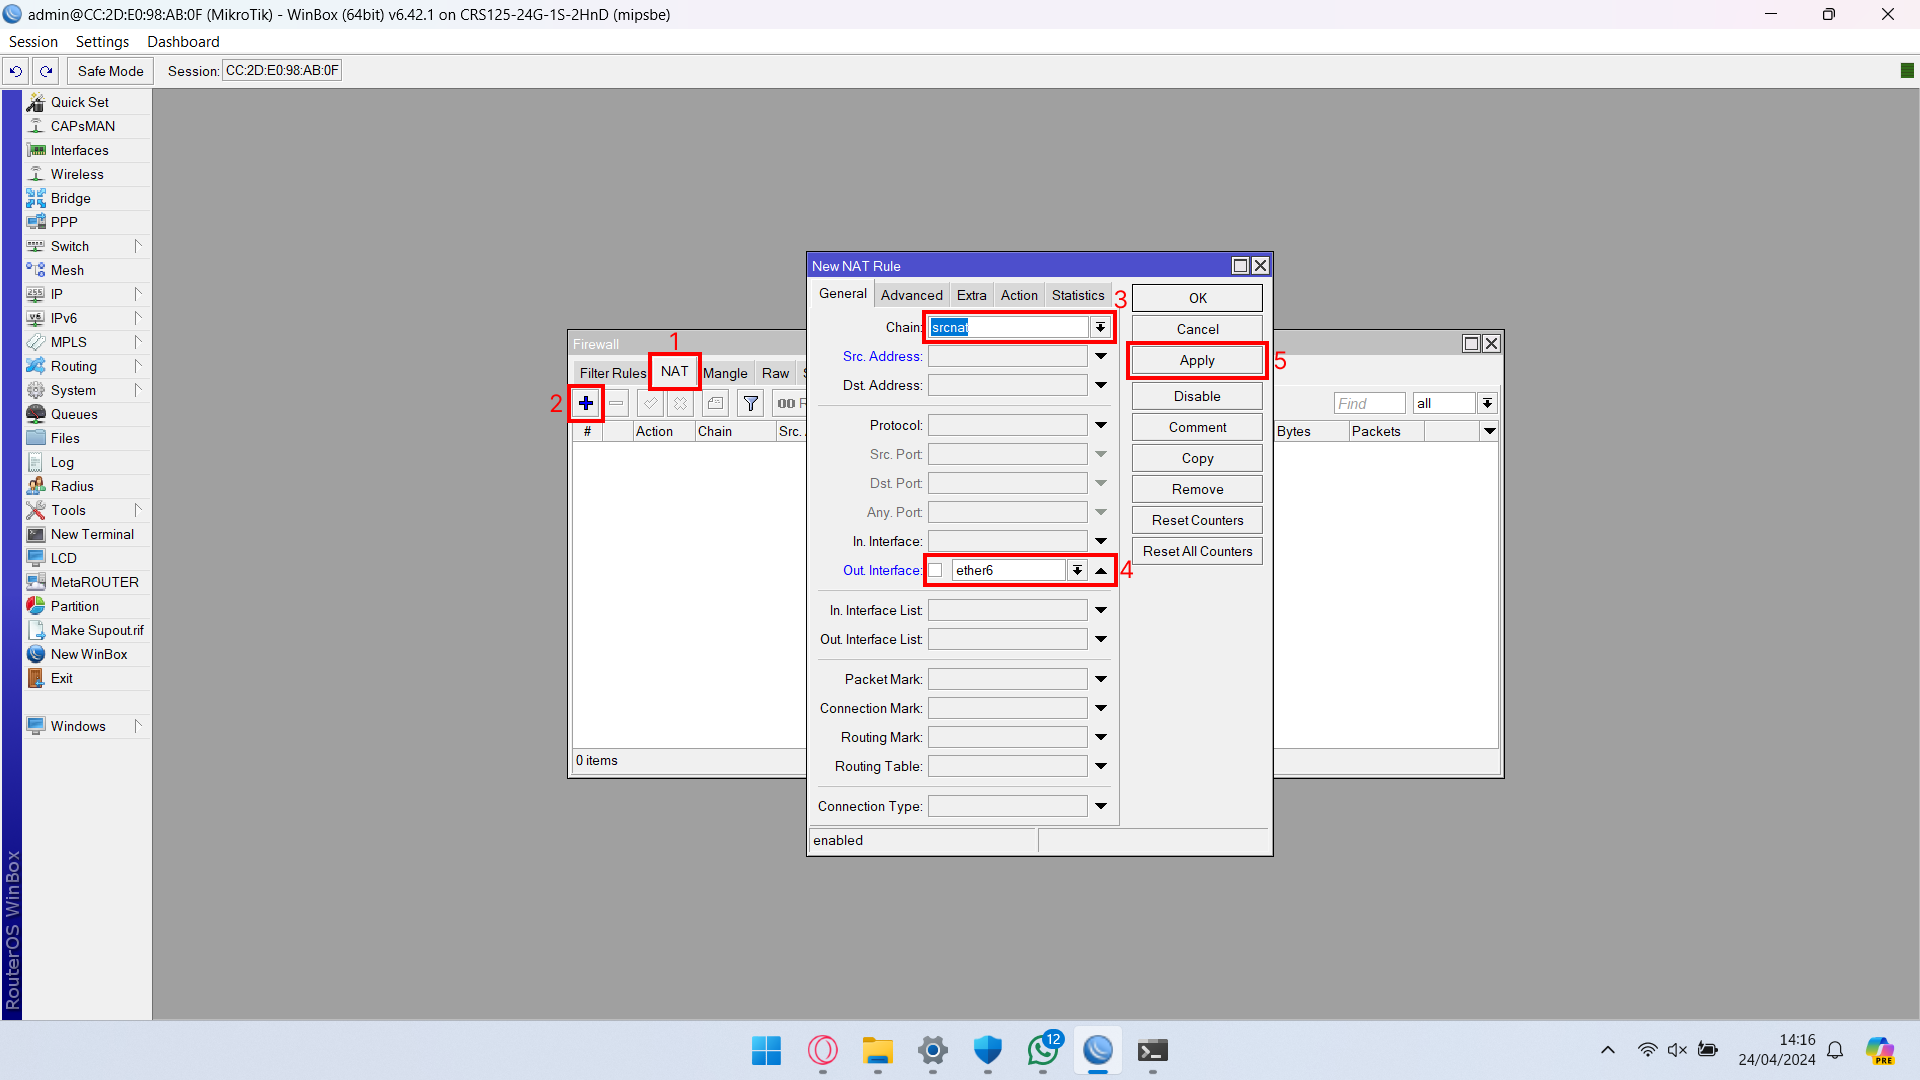
\includegraphics[width=0.8\linewidth]{P3/img/Step 13.png}
			\caption{Step 13.1}
			\label{fig:Step 13.1}
		\end{figure}
        \begin{figure}[H]
			\centering
			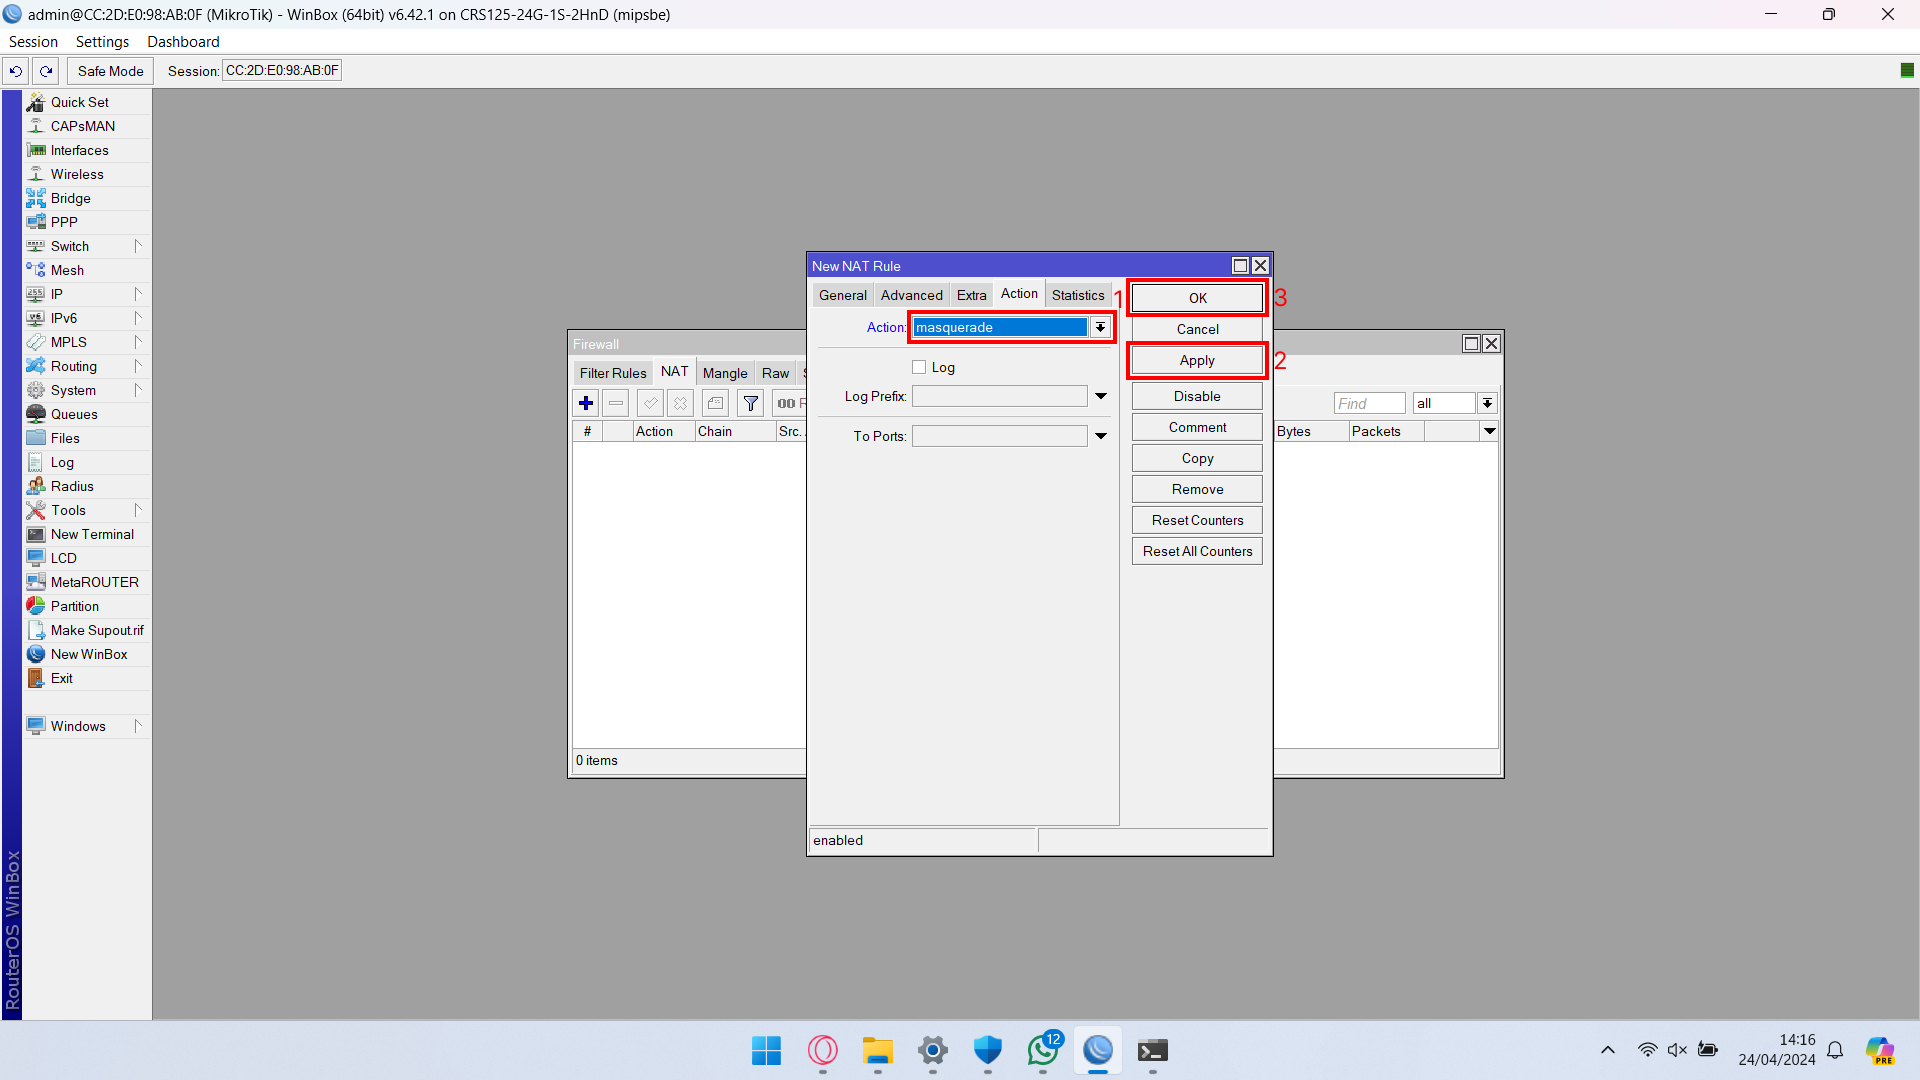
\includegraphics[width=0.8\linewidth]{P3/img/Step 14.png}
			\caption{Step 13.2}
			\label{fig:Step 14.2}
		\end{figure}
        \item Lakukan test ping ke 8.8.8.8 untuk memastikan PC sudah terhubung dengan jaringan luar.
        \begin{figure}[H]
			\centering
			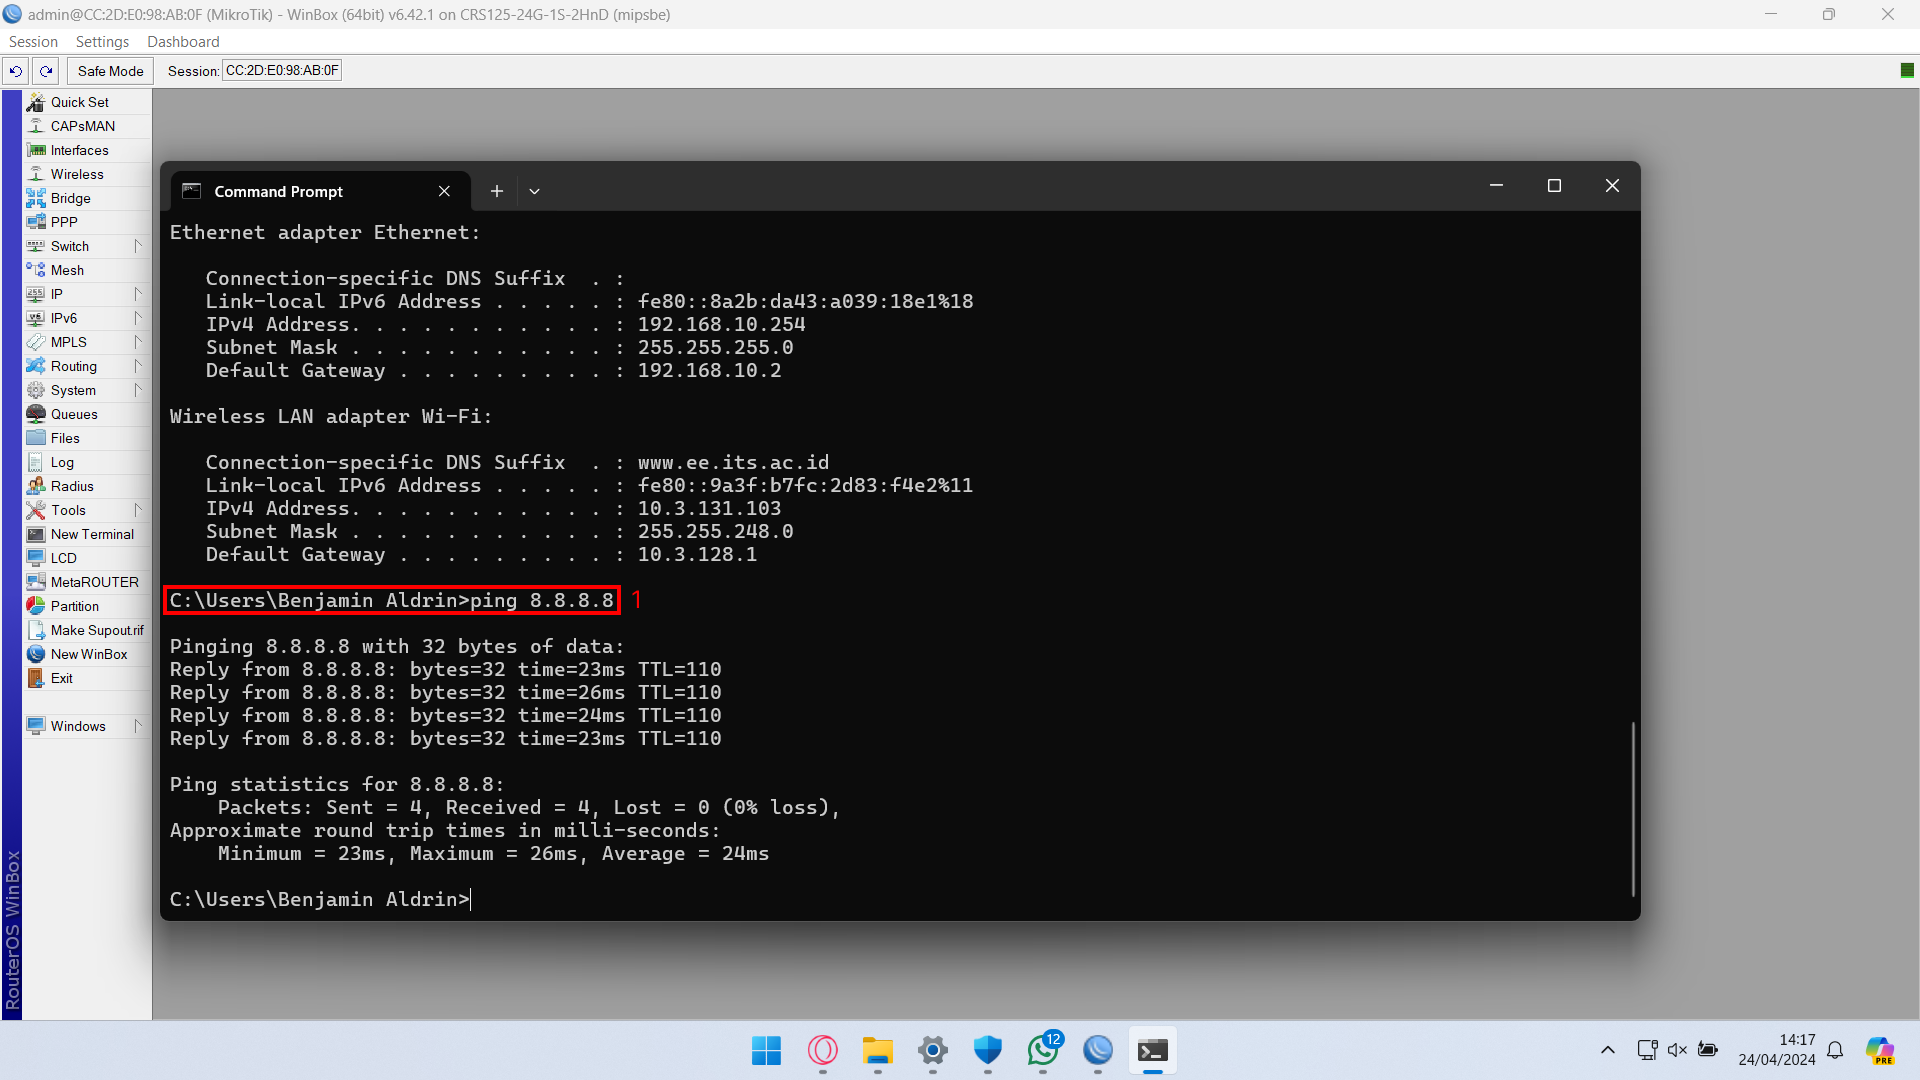
\includegraphics[width=0.8\linewidth]{P3/img/Step 15.png}
			\caption{Step 14}
			\label{fig:Step 14}
		\end{figure}
        \item Lakukan test bandwidth menggunakan SPEEDTEST melalui search engine PC.
        \begin{figure}[H]
			\centering
			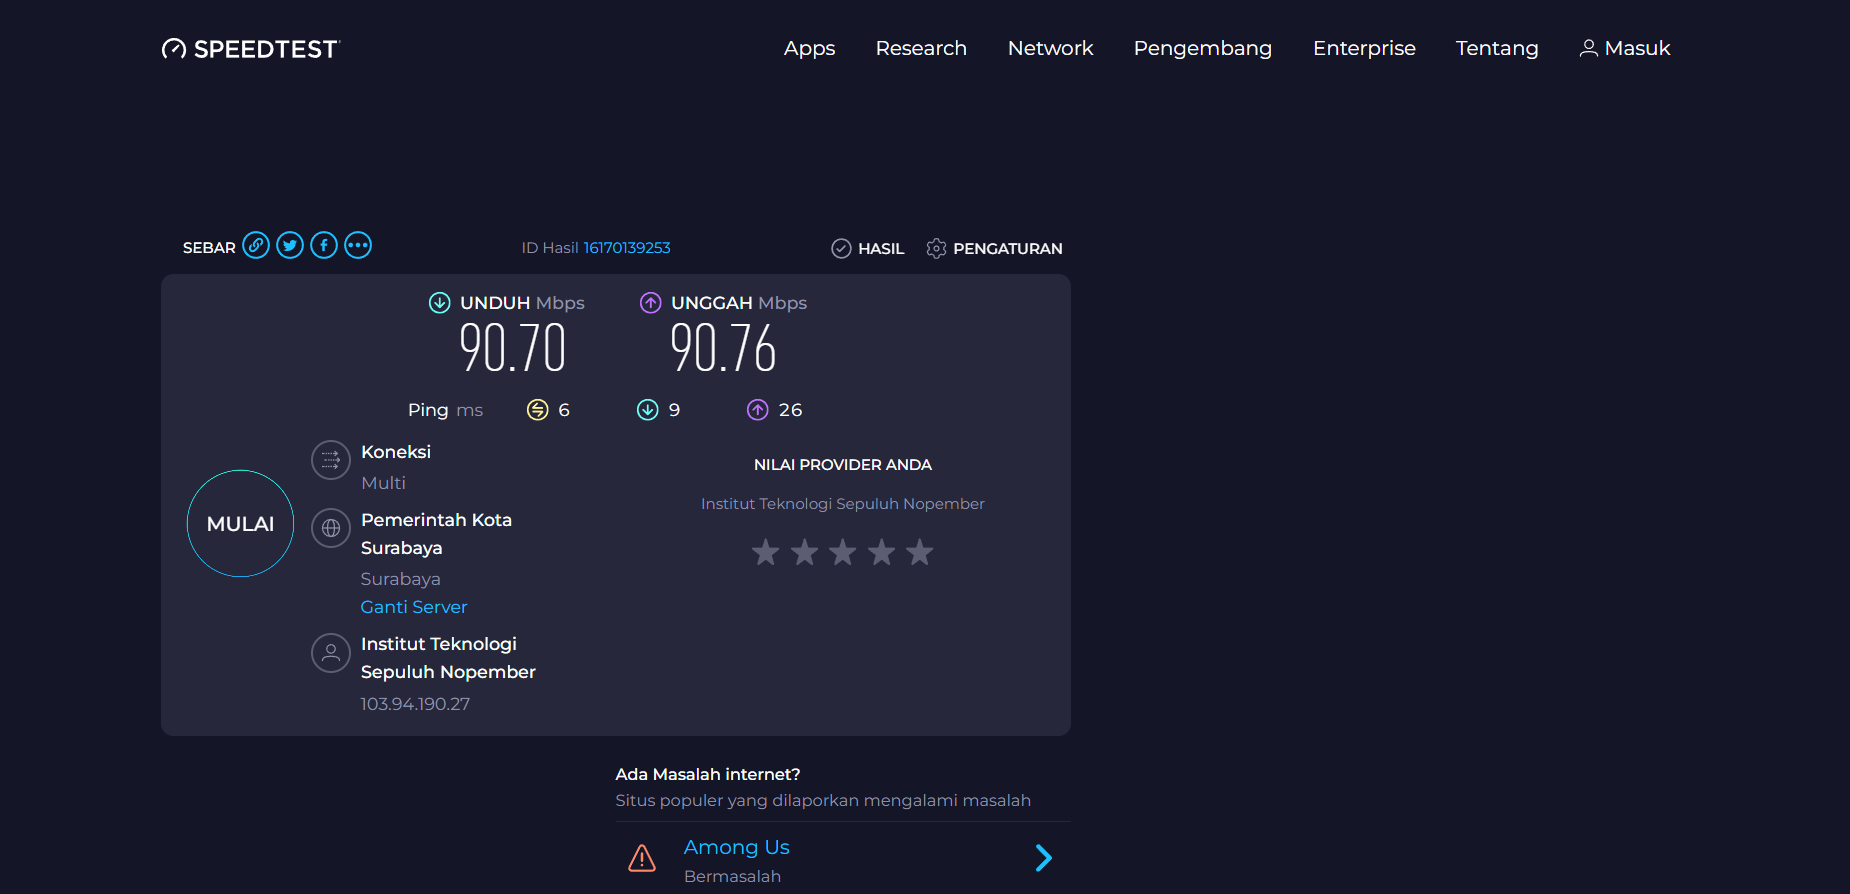
\includegraphics[width=0.8\linewidth]{P3/img/Step 16.png}
			\caption{Step 15}
			\label{fig:Step 15}
		\end{figure}
        \item Lakukan pembatasan bandwidht menggunakan Queues. Klik Queues,  Klik Queues > Tambahkan Queue List > Isi Nama perangkat yang ingin dibatasi bandwidthnya > Isi target dengan IP address PC (dapat dilihat melalui ipconfig) > Batasi Target Uploadnya menjadi 1M > Batasi Target Downloadnya menjadi 1M > Klik Apply > Klik OK.
        \begin{figure}[H]
			\centering
			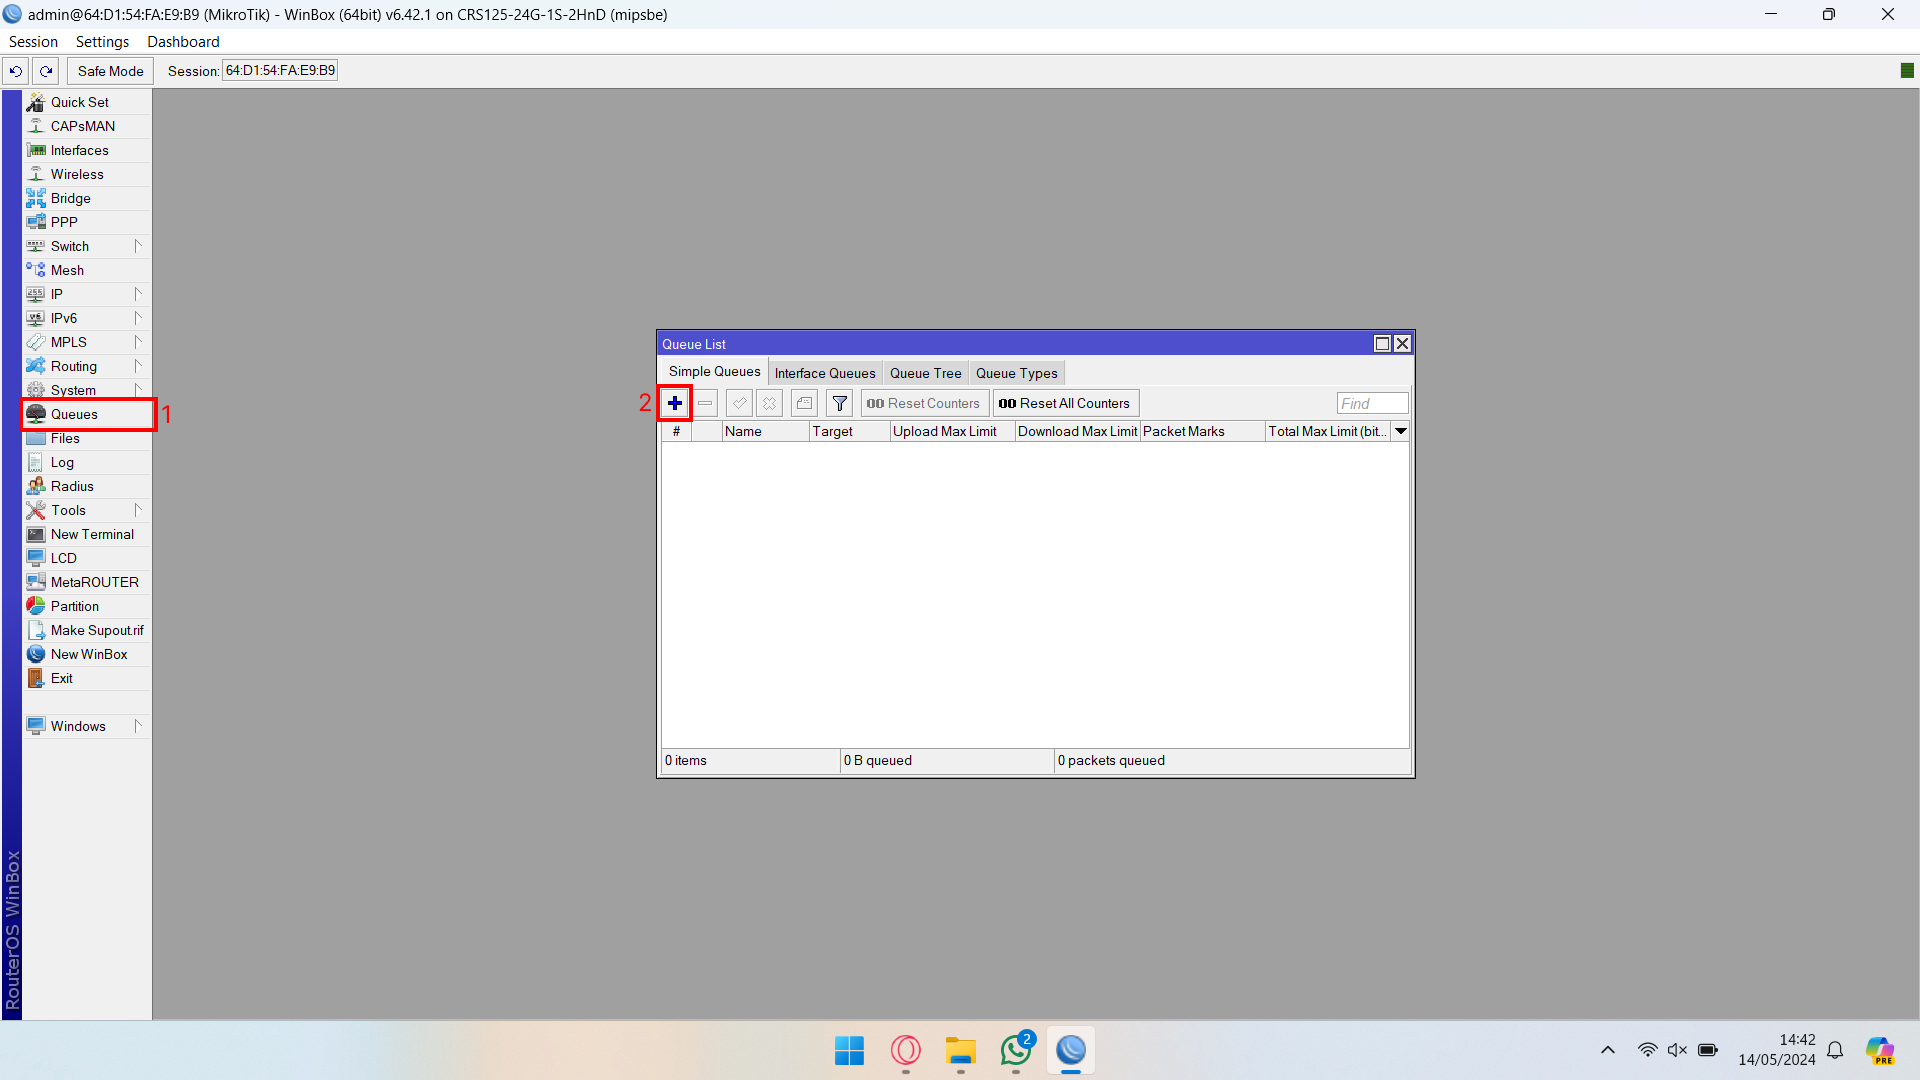
\includegraphics[width=0.8\linewidth]{P3/img/Step 17.png}
			\caption{Step 16.1}
			\label{fig:Step 16.1}
		\end{figure}
        \begin{figure}[H]
			\centering
			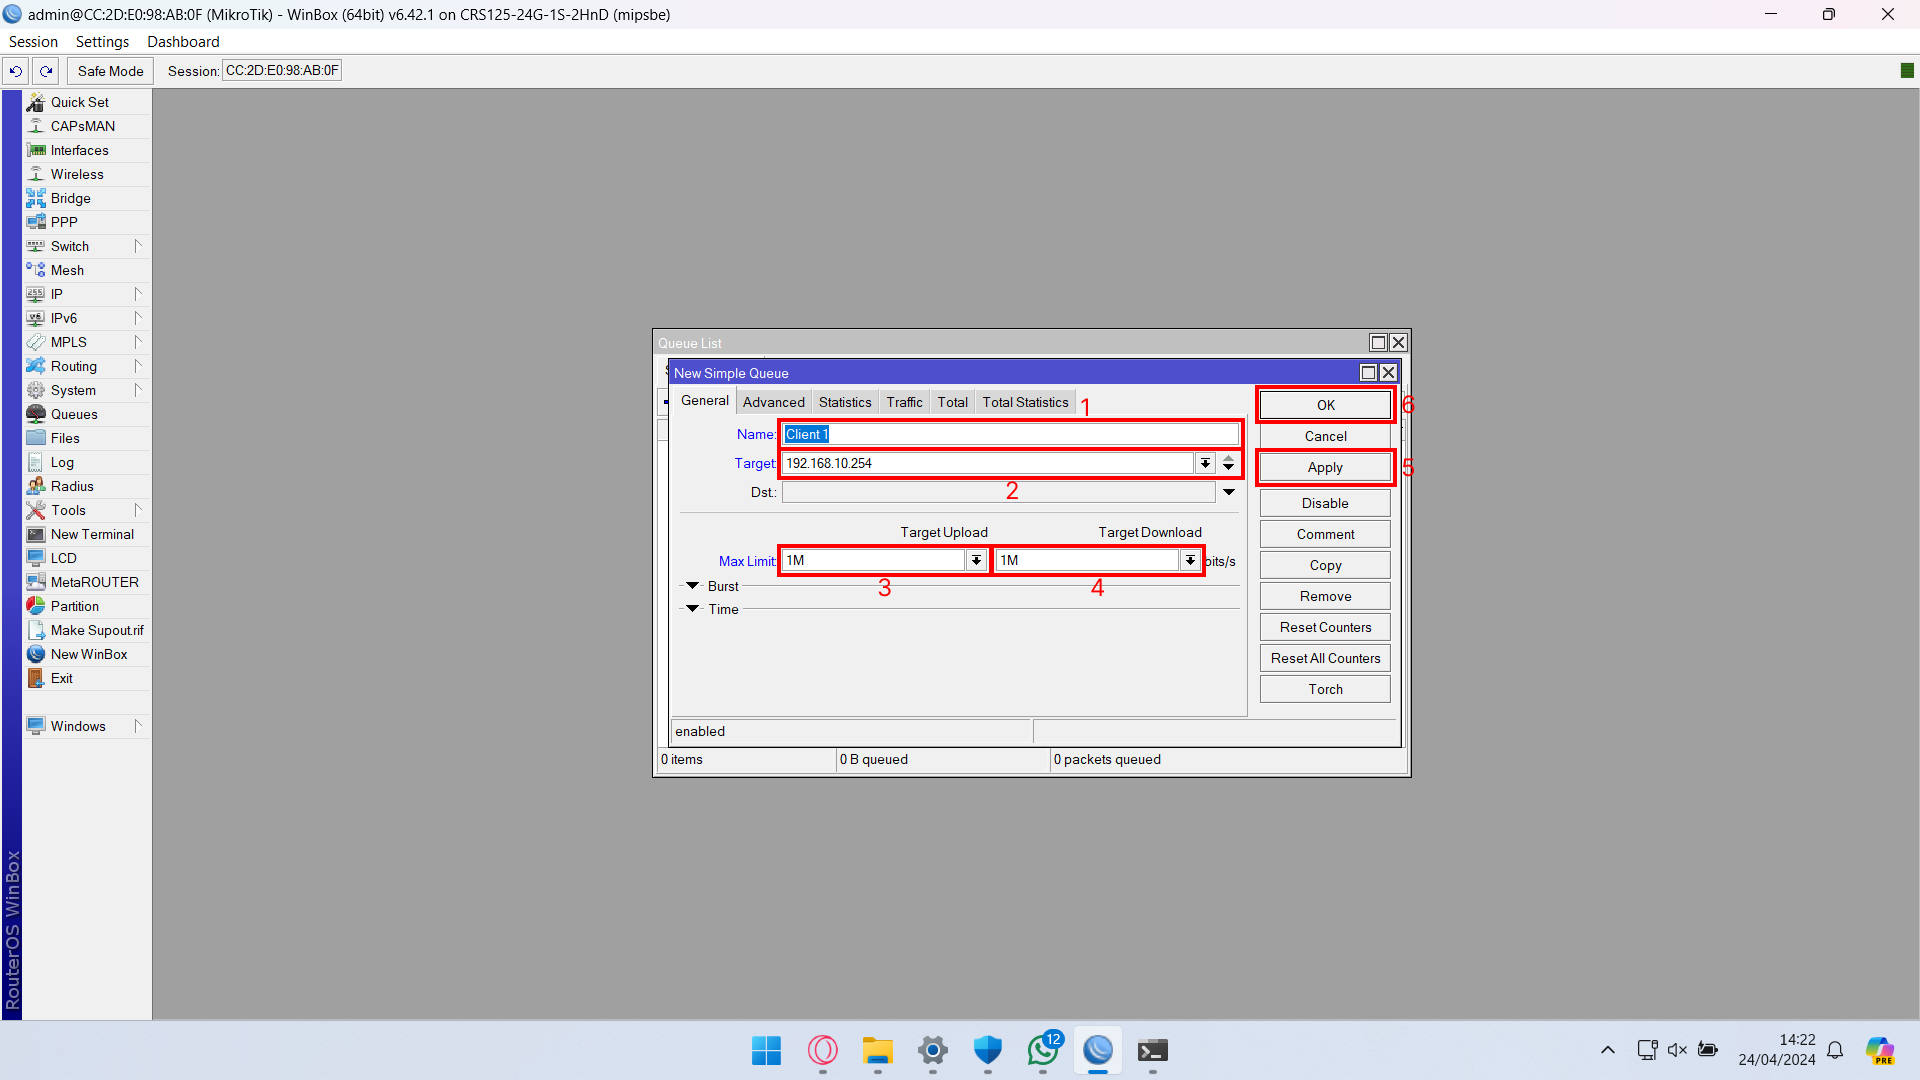
\includegraphics[width=0.8\linewidth]{P3/img/Step 18.png}
			\caption{Step 16.2}
			\label{fig:Step 16.2}
		\end{figure}
        \item Lakukan test bandwidth kembali menggunakan SPEEDTEST melalui search engine PC.
        \begin{figure}[H]
			\centering
			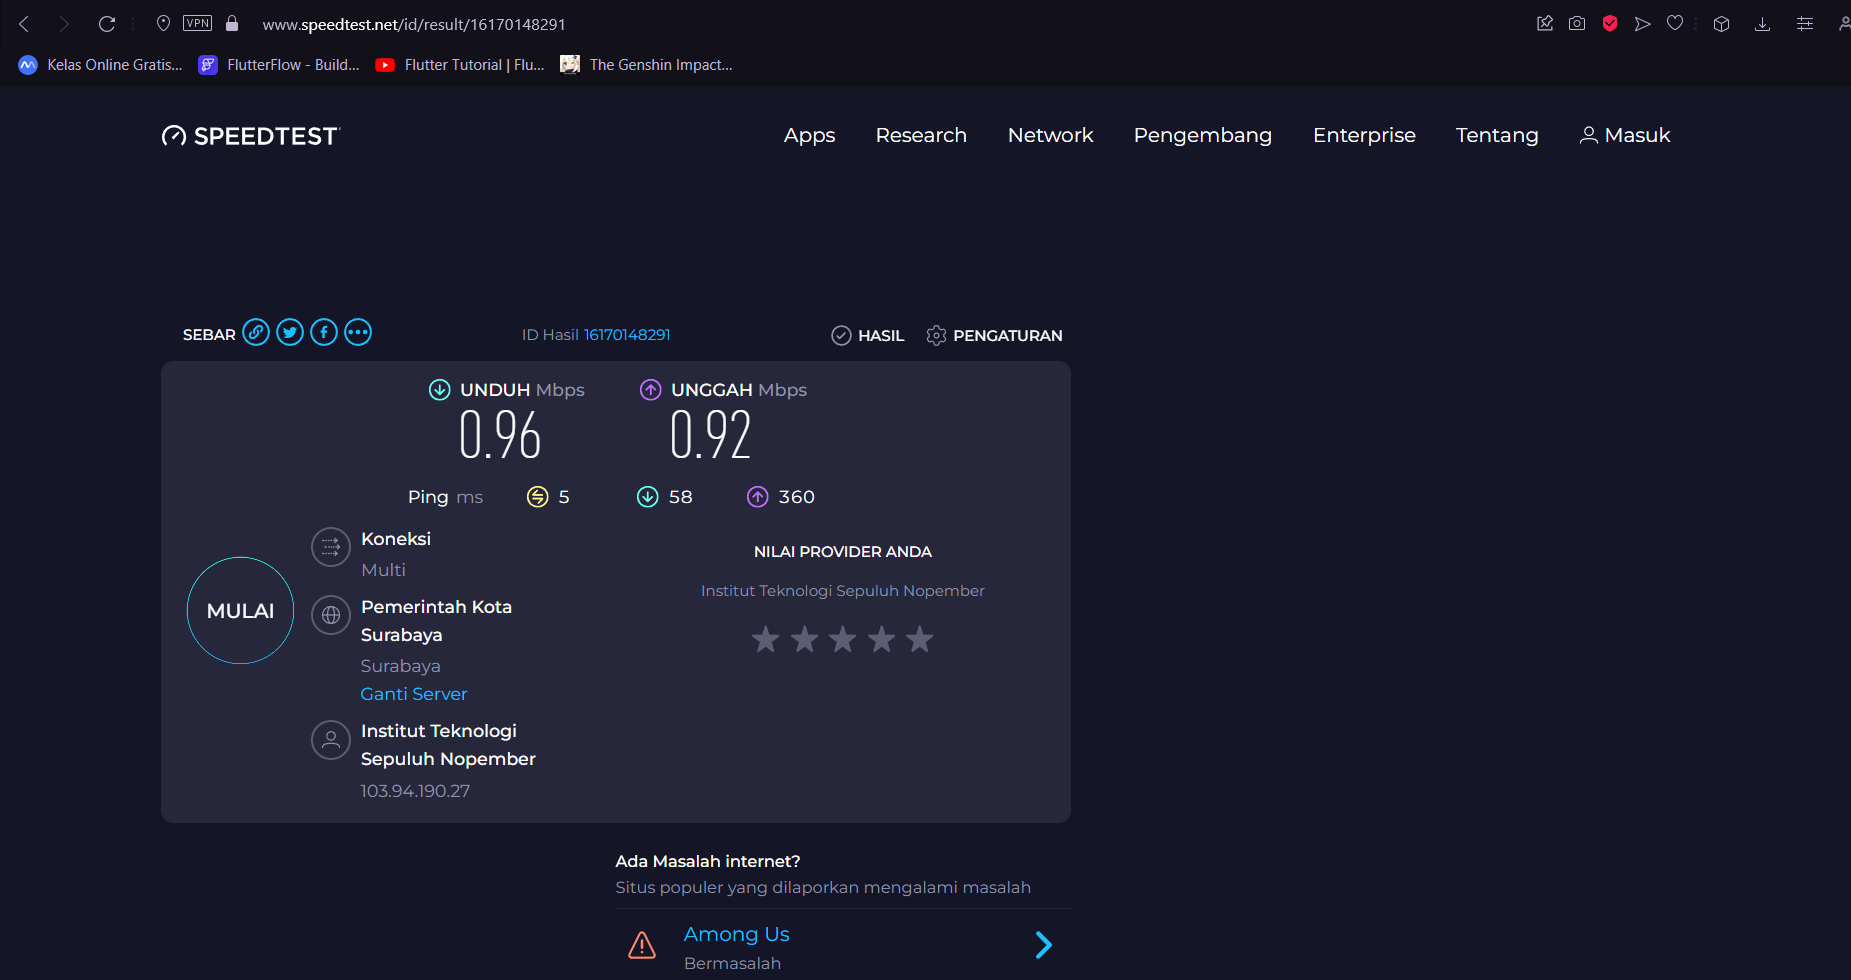
\includegraphics[width=0.8\linewidth]{P3/img/Step 19.png}
			\caption{Step 17}
			\label{fig:Step 17}
		\end{figure}
    \end{enumerate}
\end{center}

%===========================================================%
\section{Hasil yang didapat}
Memahami dan mengkonfigurasi routing dinamis RIP dengan tepat.

%===========================================================%
\section{Kesimpulan}
Dalam mengkonfigurasi routing RIP, diperlukan pemahaman dasar mengenai setting IP Address dan Subnetting, dan juga diperlukan ketelitian dan fokus agar berhasil
